\chapter{Preliminaries}
	In this chapter we discuss the groundwork for the upcoming topics. Along with these subjects, basic knowledge from linear algebra is required.

	\section{Complex Numbers}
		One of the underlying principles of \ac{QM} and therefore \ac{QC}, too, are complex numbers. This section summarizes some results for them \emph{very briefly.}

		Let \( z = a + ib \in \C \) be a complex number with the real and imaginary components \( \Re(z) = a, \Im(z) = b \in \R \). Its magnitude is
		\begin{equation}
			\lvert z \rvert \coloneqq \sqrt{a^2 + b^2} = \sqrt{z z^\ast}
		\end{equation}
		with the \emph{complex conjugate} \( z^\ast = a - ib \). The complex conjugate is distributive over addition and multiplication\footnote{For other useful properties, see \url{https://en.wikipedia.org/wiki/Complex_conjugate\#Properties}.}, i.e., \( (z_1 + z_2)^\ast = z_1^\ast + z_2^\ast \) and \( (z_1 z_2)^\ast = z_1^\ast z_2^\ast \) holds for two complex numbers \( z_1, z_2 \in \C \). Any complex number can also be written in polar form \( z = r e^{i \varphi} \) with magnitude
		\begin{equation}
			\lvert z \rvert = \sqrt{z z^\ast} = \sqrt{r e^{i \varphi} r e^{-i \varphi}} = \sqrt{r^2 e^{i \varphi - i \varphi}} = \sqrt{r^2} = \lvert r \rvert.
		\end{equation}
		\begin{definition}[\(n\)-th Root of Unity]
			We call the special complex number \( \omega_n = e^{2 \pi i / n} \) the \emph{\(n\)-th root of unity.}
		\end{definition}
		\begin{theorem}[Power Sum of \(n\)-th Roots of Unity]
			Let \( \omega_n \) be the \(n\)-th root of unity with \( n > 1 \). Then \( \sum_{k = 0}^{n - 1} \omega_n^k = 0 \).
		\end{theorem}
		\begin{proof}
			\begin{equation}
				\sum_{k = 0}^{n - 1} \omega_n^k
					= \frac{1 - \omega_n^n}{1 - \omega_n}
					= \frac{1 - e^{2 i \pi}}{1 - \omega_n}
					= \frac{1 - 1}{1 - \omega_n}
					= \frac{0}{1 - \omega_n}
					= 0
			\end{equation}
		\end{proof}
	% end

	\section{Continued Fraction Expansion}
		Let \( x \in (0, 1) \) be a real number\footnote{Note that the restriction on the interval \( (0, 1) \) is purely for convenience as we only have \(x\)'s between zero and one down the line. It is also possible to extend \aclp{CFE} to \(\R\).}. Then we can express this number as its \emph{\ac{CFE}}
		\begin{equation}
			x = \frac{1}{a_0 + \frac{1}{a_1 + \frac{1}{a_2 + \cdots}}}
		\end{equation}
		where \( a_0, a_1, \dots \in \N^+ \). The \ac{CFE} of \(x\) is finite iff \(x\) is rational. The sums
		\begin{align}
			\frac{1}{a_0} &&
			\frac{1}{a_0 + \frac{1}{a_1}} &&
			\frac{1}{a_0 + \frac{1}{a_1 + \frac{1}{a_2}}} &&
			\cdots
		\end{align}
		are called \emph{partial sums.} For calculating \( a_0, a_1, \dots \), let
		\begin{align}
			x_0 &\coloneqq \frac{1}{a_0 + \frac{1}{a_1 + \frac{1}{a_2 + \cdots}}} &
			x_1 &\coloneqq \frac{1}{a_1 + \frac{1}{a_2 + \cdots}} &
			x_2 &\coloneqq \frac{1}{a_2 + \cdots} &
			\cdots
		\end{align}
		then the coefficients are \( a_i = [1 / x_i] \), where the brackets indicate the integral part, i.e., the part in front of the decimal. If for any \(j\), \(x_j = 0\), the \ac{CFE} terminates and the number is exactly represented.

		\begin{example}
			Let \( x = \num{11490} / 2^{14} \approx 0.701294 \). Then the \ac{CFE} is calculated as follows:
			\begin{center}
				\begin{tabular}{c|ccc}
					\toprule
					 \(i\)  &	\(x_i\)	 &  \(1 / x_i\)  & \(a_i\)  \\ \midrule
					\num{0} & \num{0.701294} & \num{1.42594} & \num{1}  \\ \bottomrule
					\num{1} & \num{0.42594}  & \num{2.34777} & \num{2}  \\ \bottomrule
					\num{2} & \num{0.34777}  & \num{2.87544} & \num{2}  \\ \bottomrule
					\num{3} & \num{0.87544}  & \num{1.14228} & \num{1}  \\ \bottomrule
					\num{4} & \num{0.14228}  & \num{7.02830} & \num{7}  \\ \bottomrule
					\num{5} & \num{0.02830}  & \num{35.3333} & \num{35} \\ \bottomrule
					\num{6} & \num{0.33333}  &	\num{3}	& \num{3}  \\ \bottomrule
					\num{7} &	\num{0}	 &			   &		  \\ \bottomrule
				\end{tabular}
			\end{center}
			The final \ac{CFE} is therefore
			\begin{equation}
				x = \frac{1}{1 + \frac{1}{2 + \frac{1}{2 + \frac{1}{1 + \frac{1}{7 + \frac{1}{35 + \frac{1}{3}}}}}}}
			\end{equation}
			with the coefficients \( (a_0, a_1, a_2, a_3, a_4, a_5, a_6) = (1, 2, 2, 1, 7, 35, 3) \).
		\end{example}
	% end
% end

\chapter{Postulates of Quantum Mechanics}
	In this chapter we discuss the postulates of \ac{QM} and some important protocols and results in \ac{QC} such as the \emph{no-cloning theorem.} This theorem states that it is impossible to copy a quantum state!

	\section{States}
		In classical computing, a bit is either \num{0} or \num{1}. A quantum bit, a \emph{qubit,} however, is more general and has the basis states \(\ket{0}\) and \(\ket{1}\). The states are formed by basis vectors \( \ket{0} = (1, 0)^\dagger \) and \( \ket{1} = (0, 1)^\dagger \). More generally, an arbitrary quantum state \(\ket{\psi}\) can be a combination of the basis states, \( \ket{\psi} = c_0 \ket{0} + c_1 \ket{1} \), a \emph{superposition} (with complex coefficients \( c_0, c_1 \in \C \)). However, the state has to be normalized, i.e., \( \lvert \braket{\psi}{\psi} \rvert^2 = 1 \). The left part of this inner product is called a \emph{bra} vector representing the conjugate transpose of the right side, the \emph{ket} vector.

		The following postulate digests this idea more formally.

		\begin{postulate}[Quantum State]
			Any closed physical system can be associated with a Hilbert space \(\mathcal{H}\). The state of the system is completely described by a state vector \( \ket{\psi} = \sum_{i = 0}^{d - 1} c_i \ket{i} \) with \( \sum_{i = 0}^{d - 1} \lvert c_i \rvert^2 = 1 \) where \( \{ \ket{i} \}_{i = 0}^{d - 1} \) forms a basis of \( \mathcal{H}^d \).
		\end{postulate}
		\begin{remark}
			The basis is not confined to the \emph{computational basis} \( \{ \ket{0}, \ket{1} \} \), although this basis is often used. It may be any other orthonormal basis of \(\mathcal{H}\), see \autoref{subsec:otherBasis}. For basis of Hilbert spaces with \(d > 2\), see \autoref{sec:composite}.
		\end{remark}

		Instead of writing out the complex coefficients \(c_0\) and \(c_1\), we can also parameterize an arbitrary superposition with angles \( \gamma, \varphi, \theta \in \R \):
		\begin{equation}
			\ket{\psi}
				= c_0 \ket{0} + c_1 \ket{1}
				= e^{i \gamma} \biggl( \cos\frac{\theta}{2} \ket{0} + e^{i \varphi} \sin\frac{\theta}{2} \ket{1} \biggr).
		\end{equation}
		However, as we will see in \autoref{sec:measurement}, a global phase such as \(e^{i \gamma}\) vanishes in all important calculations as \( e^{i \gamma} e^{-i \gamma} = 1 \). Hence, we can also parameterize any state with just two angles \( \varphi \in (0, 2\pi] \) and \( \theta \in (0, \pi] \):
		\begin{equation}
			\ket{\psi} = \cos\frac{\theta}{2} \ket{0} + e^{i \varphi} \sin\frac{\theta}{2} \ket{1}.
		\end{equation}
		Checking that this state is actually normalized is straightforward:
		\begin{align}
			\braket{\psi}{\psi}
				&= \biggl( \cos\frac{\theta}{2} \bra{0} + e^{-i \varphi} \sin\frac{\theta}{2} \bra{1} \biggr) \biggl( \cos\frac{\theta}{2} \ket{0} + e^{i \varphi} \sin\frac{\theta}{2} \ket{1} \biggr) \\
				&= \cos\frac{\theta}{2} \bra{0} + e^{-i \varphi} \sin\frac{\theta}{2} \bra{1} \biggr) \biggl( \cos\frac{\theta}{2} \ket{0} + e^{i \varphi} \sin\frac{\theta}{2} \ket{1} \biggr) \\
				&= \cos^2\frac{\theta}{2} \underbrace{\braket{0}{0}}_{= 1}
					+ e^{i \varphi} \cos\frac{\theta}{2} \sin\frac{\theta}{2} \underbrace{\braket{0}{1}}_{= 0}
					+ e^{-i \varphi} \cos\frac{\theta}{2} \sin\frac{\theta}{2} \underbrace{\braket{1}{0}}_{= 0}
					+ e^{i \varphi} e^{-i \varphi} \sin\frac{\theta}{2} \sin\frac{\theta}{2} \underbrace{\braket{1}{1}}_{= 1} \\
				&= \cos^2\frac{\theta}{2} + \sin^2\frac{\theta}{2}
			 = 1.
		\end{align}
		Note that in this case \( \braket{\psi}{\psi} = 1 \), so \( \lvert \braket{\psi}{\psi} \rvert^2 = 1 \) holds, too, and we can drop the absolute-square. In most of the following discussions where we need explicit parametrization, we confine ourselves to real coefficients, i.e., \(\varphi = 0\). This simplifies the discussion as now there is only one parameter \(\theta\).
	% end

	\section{Evolution}
		The evolution of quantum states, i.e., how they pass between states, is described by linear transformations \(U\), also called \emph{gates.} These gates transform a quantum state \(\ket{\psi}\) into another quantum state \(\ket{\psi'}\). In quantum circuits, we denote an application of \(U_1\) and then \(U_2\) to a state \(\ket{\psi}\), i.e., \( U_2 U_1 \ket{\psi} \), as:
		\begin{equation}
			\Qcircuit @C=1em @R=1em {
				\lstick{\ket{\psi}} & \gate{U_1} & \gate{U_2} & \rstick{U_2 U_1 \ket{\psi}} \qw
			}
		\end{equation}

		\begin{postulate}[State Evolution]
			The evolution \( \ket{\psi(t_0)} \overset{U}{\longto} \ket{\psi(t)} \) of a closed physical system is described by a unitary transformation \( U U^\dagger = \ID \).
		\end{postulate}

		\begin{theorem}[Unitarity of Quantum Gates]
			A linear quantum gate \(U\) is unitary, i.e., \( U U^\dagger = \ID \).
		\end{theorem}
		\begin{proof}
			\todo{Proof: Unitarity of Quantum Gates}
%			Let \( U = \begin{bmatrix} u_{00} & u_{01} \\ u_{10} & u_{11} \end{bmatrix} \) be an arbitrary gate. Then application of this gate to \(\ket{0}\), \(\ket{1}\), \(\bra{0}\), and \(\bra{1}\) must produce a \emph{normalized} quantum state:
%			\begin{align}
%				\lVert U \ket{0} \rVert_2^2 &= \lvert u_{00} \rvert^2 + \lvert u_{10} \rvert^2 \overset{!}{=} 1 &
%				\lVert U \ket{1} \rVert_2^2 &= \lvert u_{01} \rvert^2 + \lvert u_{11} \rvert^2 \overset{!}{=} 1 \\
%				\lVert \bra{0} U \rVert_2^2 &= \lvert u_{00} \rvert^2 + \lvert u_{01} \rvert^2 \overset{!}{=} 1 &
%				\lVert \bra{1} U \rVert_2^2 &= \lvert u_{10} \rvert^2 + \lvert u_{11} \rvert^2 \overset{!}{=} 1
%			\end{align}
%			From these four constraints it follows that the columns and rows of \(U\) must be normalized. It remains to be shown that they are orthogonal. The application of \(U\) to \( \ket{+} = (\ket{0} + \ket{1}) / \sqrt{2} \) and \( \ket{+_y} = (\ket{0} + i \ket{1}) / \sqrt{2} \) must produce normalized states, too:
%			\begin{align}
%				\lVert U \ket{+} \rVert_2^2
%					&= \frac{1}{2} \bigl( \lvert u_{00} + u_{01} \rvert^2 + \lvert u_{10} + u_{11} \rvert^2 \bigr) \\
%					&= \frac{1}{2} \bigl( (u_{00} + u_{01}) (u_{00} + u_{01})^\ast + (u_{10} + u_{11}) (u_{10} + u_{11})^\ast \bigr) \\
%					&= \frac{1}{2} \bigl( (u_{00} + u_{01}) (u_{00}^\ast + u_{01}^\ast) + (u_{10} + u_{11}) (u_{10}^\ast + u_{11}^\ast) \bigr) \\
%					&= \frac{1}{2} \bigl( u_{00} (u_{00}^\ast + u_{01}^\ast) + u_{01} (u_{00}^\ast + u_{01}^\ast) + u_{10} (u_{10}^\ast + u_{11}^\ast) + u_{11} (u_{10}^\ast + u_{11}^\ast) \bigr) \\
%					&= \frac{1}{2} \bigl( u_{00} u_{00}^\ast + u_{00} u_{01}^\ast + u_{01} u_{00}^\ast + u_{01} u_{01}^\ast + u_{10} u_{10}^\ast + u_{10} u_{11}^\ast + u_{11} u_{10}^\ast + u_{11} u_{11}^\ast \bigr) \\
%					&= \frac{1}{2} \bigl( \underbrace{\lvert u_{00} \rvert^2 + \lvert u_{01} \rvert^2}_{= 1} + \underbrace{\lvert u_{10} \rvert^2 + \lvert u_{11} \rvert^2}_{= 1} + u_{00} u_{01}^\ast + u_{01} u_{00}^\ast + u_{10} u_{11}^\ast + u_{11} u_{10}^\ast \bigr) \\
%					&= 1 + \frac{1}{2} \bigl( u_{00} u_{01}^\ast + u_{01} u_{00}^\ast + u_{10} u_{11}^\ast + u_{11} u_{10}^\ast \bigr) \overset{!}{=} 1 \\
%				\lVert U \ket{+_y} \rVert_2^2
%					&= \frac{1}{2} \bigl( \lvert u_{00} + i u_{01} \rvert^2 + \lvert u_{10} + i u_{11} \rvert^2 \bigr) \\
%					&= \frac{1}{2} \bigl( (u_{00} + i u_{01}) (u_{00} + i u_{01})^\ast + (u_{10} + i u_{11}) (u_{10} + i u_{11})^\ast \bigr) \\
%					&= \frac{1}{2} \bigl( (u_{00} + i u_{01}) (u_{00}^\ast - i u_{01}^\ast) + (u_{10} + i u_{11}) (u_{10}^\ast - i u_{11}^\ast) \bigr) \\
%					&= \frac{1}{2} \bigl( u_{00} (u_{00}^\ast - i u_{01}^\ast) + i u_{01} (u_{00}^\ast - i u_{01}^\ast) + u_{10} (u_{10}^\ast - i u_{11}^\ast) + i u_{11} (u_{10}^\ast - i u_{11}^\ast) \bigr) \\
%					&= \frac{1}{2} \bigl( u_{00} u_{00}^\ast - i u_{00} u_{01}^\ast + i u_{01} u_{00}^\ast + u_{01} u_{01}^\ast + u_{10} u_{10}^\ast - i u_{10} u_{11}^\ast + i u_{11} u_{10}^\ast + u_{11} u_{11}^\ast \bigr) \\
%					&= \frac{1}{2} \bigl( \underbrace{\lvert u_{00} \rvert^2 + \lvert u_{01} \rvert^2}_{= 1} + \underbrace{\lvert u_{10} \rvert^2 + \lvert u_{11} \rvert^2}_{= 1} - i u_{00} u_{01}^\ast + i u_{01} u_{00}^\ast - i u_{10} u_{11}^\ast + i u_{11} u_{10}^\ast \bigr) \\
%					&= 1 + \frac{1}{2} \bigl( - i u_{00} u_{01}^\ast + i u_{01} u_{00}^\ast - i u_{10} u_{11}^\ast + i u_{11} u_{10}^\ast \bigr) \overset{!}{=} 1
%			\end{align}
		\end{proof}

		\subsection{Gates}
			% TODO: Interpretation of unitaries as rotations in the Bloch sphere.
			In this section we collect the most important single-qubit gates. They are summarized in \autoref{tab:gates} and their semantics are given in the caption.

			\begin{theorem}[Decomposition of Two-By-Two Unitary Matrices]  \label{th:twoByTwoDecomposition}
				Every unitary matrix \( U \in \C^{2 \times 2} \) can be decomposed into three rotations as \( U = e^{i \alpha} R_z(\beta) R_y(\gamma) R_z(\delta) \).
			\end{theorem}

			From this theorem, one might think that it is necessary to implement every rotation in the lab for a universal quantum computer. Fortunately, this is not the case! As we will see in \autoref{c:universality}, only three gates are necessary to implement arbitrary rotations.

			\begin{table}
				\centering
				\begin{tabular}{l|ll|ll}
					\toprule
						  \(U\)
						& \(U \ket{0}\)
						& \(U \ket{1}\)
						& \(U \ket{+}\)
						& \(U \ket{-}\)
						\\ \midrule
						  \( X = \begin{bmatrix} 0 & 1 \\ 1 & 0 \end{bmatrix} = H Z H \)
						& \(  \ket{1} \)
						& \(  \ket{0} \)
						& \(  \ket{+} \)
						& \( -\ket{-} \)
						\\
						  \( Y = \begin{bmatrix} 0 & -i \\ i & 0 \end{bmatrix} \equiv X Z \)
						& \(  i \ket{1} \)
						& \( -i \ket{0} \)
						& \( -i \ket{-} \)
						& \(  i \ket{+} \)
						\\
						  \( Z = \begin{bmatrix} 1 & 0 \\ 0 & -1 \end{bmatrix} \)
						& \(  \ket{0} \)
						& \( -\ket{1} \)
						& \(  \ket{-} \)
						& \(  \ket{+} \)
						\\
						  \( H = \frac{1}{\sqrt{2}} \begin{bmatrix} 1 & 1 \\ 1 & -1 \end{bmatrix} \)
						& \( \ket{+} \)
						& \( \ket{-} \)
						& \( \ket{0} \)
						& \( \ket{1} \)
						\\
						  \( R_y(\gamma) = \begin{bmatrix} c_\gamma & -s_\gamma \\ s_\gamma & c_\gamma \end{bmatrix} \)
						& \(  c_\gamma \ket{0} + s_\gamma \ket{1} \)
						& \( -s_\gamma \ket{0} + c_\gamma \ket{1} \)
						& \(  c_\gamma \ket{+} - s_\gamma \ket{-} \)
						& \(  s_\gamma \ket{+} + c_\gamma \ket{-} \)
						\\
						  \( R_z(\beta) = \begin{bmatrix} e^{i \beta / 2} & 0 \\ 0 & e^{-i \beta / 2} \end{bmatrix} \)
						& \( e^{ i \beta / 2} \ket{0} \)
						& \( e^{-i \beta / 2} \ket{1} \)
						& \( e^{ i \beta / 2} \ket{0} + e^{-i \beta / 2} \ket{1} \)
						& \( e^{ i \beta / 2} \ket{0} - e^{-i \beta / 2} \ket{1} \)
						\\
					\bottomrule
				\end{tabular}
				\caption[Common Single-Qubit Gates]{Common qubit gates and their effect on the computational and Hadamard basis. For brevity, let \( c_\gamma \coloneqq \cos(\gamma / 2) \) and \( s_\gamma \coloneqq \sin(\gamma / 2) \). The gates have the following effects in the computational basis: \(X\) implements a logical not, \(Y\) combines a phase-flip and logical not, \(Z\) implements a phase-flip, \(H\) creates an equal superposition, \(R_y(\gamma)\) rotates around an arbitrary angle \(\gamma\), and \(R_z(\beta)\) adds a phase. In Hadamard basis, the gates have the following effects: \(X\) implement a phase-flip, \(Y\) combined a phase-flip and logical not, \(Z\) implements a logical not, \(H\) creates an equal superposition, \(R_y(\gamma)\) rotates around an arbitrary angle \(\gamma\), and \(R_z(\beta)\) adds a phase.}
				\label{tab:gates}
			\end{table}
		% end
	% end

	\section{Measurement}
		\label{sec:measurement}

		We will now discuss the last postulate of \ac{QM} which is concerned with \emph{measurements.} The central result is that measuring a quantum system is inherently \emph{probabilistic,} i.e., the outcome of a measurement is not deterministic and truly random. For any quantum state \( \ket{\psi} \), the probability of measuring an outcome \(v_i\) is given by the absolute-square of the inner product between the "measurement state" \(\ket{v_i}\) and the state \(\ket{\psi}\):
		\begin{equation}
			P(i) = \lvert \ip{v_i}{\psi} \rvert^2.
		\end{equation}
		The value of this inner product (without the absolute-square) is called the \emph{probability amplitude} and can be negative or even complex. Immediately after a measurement, the state \(\ket{\psi}\) collapses into a post-measurement state \(\ket{\psi'}\). This post-measurement state is
		\begin{equation}
			\ket{\psi'} = \frac{M_i \ket{\psi}}{N_i}
		\end{equation}
		where \( M_i = \op{v_i}{v_i} \) and \( N_i = \sqrt{P(i)} \) are the \emph{measurement operator} and \emph{normalization constant,} respectively. These results are digested in the following postulate.

		\begin{postulate}[Quantum Measurement]
			Quantum measurements are described by a collection of measurement operators \( \{ M_i \} \) where \(i\) indicated the outcome of the experiment. Let \(\ket{\psi}\) be the state before the measurement, then the state immediately after the measurement is \( \ket{\psi'} = M_i \ket{\psi} / N_i \) where \( N = \sqrt{P(i)} \) is for normalization.
		\end{postulate}

		\begin{theorem}[Measurement of Pure Quantum States]
			For \emph{pure} states \(\ket{\psi}\), the post-measurement state \(\ket{\psi'}\) after a measurement of \(\ket{v_i}\) is \(\ket{\psi'} = \ket{v_i}\).
		\end{theorem}
		\begin{proof}
			\begin{equation}
				\frac{M_i \ket{\psi}}{N_i}
					= \frac{\op{v_i}{v_i} \ket{\psi}}{\sqrt{P(i)}}
					= \frac{\op{v_i}{v_i} \ket{\psi}}{\sqrt{\lvert \ip{v_i}{\psi} \rvert^2}}
					= \frac{\ket{v_i} \ip{v_i}{\psi}}{\lvert \ip{v_i}{\psi} \rvert}
					= \ket{v_i} \frac{\ip{v_i}{\psi}}{\lvert \ip{v_i}{\psi} \rvert}
					\equiv \ket{v_i}
			\end{equation}
		\end{proof}
	% end

	\section{Composite Systems and Tensor Products}
		\label{sec:composite}

		As in classical computing where we are concerned with more than one bit, \ac{QC} also works with more than one qubit. The formalism for this are \emph{tensor products} \( \mathcal{H}^2 \otimes \mathcal{H}^2 \) between the Hilbert spaces of the individual qubits. Its basis vectors are also constructed using tensor products:
		\begin{align}
			\ket{0} \otimes \ket{0} &= \begin{bmatrix} 1 \\ 0 \\ 0 \\ 0 \end{bmatrix} &
			\ket{0} \otimes \ket{1} &= \begin{bmatrix} 0 \\ 1 \\ 0 \\ 0 \end{bmatrix} &
			\ket{1} \otimes \ket{0} &= \begin{bmatrix} 0 \\ 0 \\ 1 \\ 0 \end{bmatrix} &
			\ket{1} \otimes \ket{1} &= \begin{bmatrix} 0 \\ 0 \\ 0 \\ 1 \end{bmatrix}
		\end{align}
		For two single-qubit operators \( A = \begin{bmatrix} a_{00} & a_{01} \\ a_{10} & a_{11} \end{bmatrix} \) and \( B = \begin{bmatrix} b_{00} & b_{01} \\ b_{10} & b_{11} \end{bmatrix} \), the tensor product is carried out as
		\begin{equation}
			A \otimes B
				= \begin{bmatrix} a_{00} & a_{01} \\ a_{10} & a_{11} \end{bmatrix} \otimes \begin{bmatrix} b_{00} & b_{01} \\ b_{10} & b_{11} \end{bmatrix}
				= \begin{bmatrix} a_{00} \begin{bmatrix} b_{00} & b_{01} \\ b_{10} & b_{11} \end{bmatrix} & a_{01} \begin{bmatrix} b_{00} & b_{01} \\ b_{10} & b_{11} \end{bmatrix} \\ a_{10} \begin{bmatrix} b_{00} & b_{01} \\ b_{10} & b_{11} \end{bmatrix} & a_{11} \begin{bmatrix} b_{00} & b_{01} \\ b_{10} & b_{11} \end{bmatrix} \end{bmatrix}
				=
					\begin{bmatrix}
						a_{00} b_{00} & a_{00} b_{01} & a_{01} b_{00} & a_{01} b_{01} \\
						a_{00} b_{10} & a_{00} b_{11} & a_{01} b_{10} & a_{01} b_{11} \\
						a_{10} b_{00} & a_{10} b_{01} & a_{11} b_{00} & a_{11} b_{01} \\
						a_{10} b_{10} & a_{10} b_{11} & a_{11} b_{10} & a_{11} b_{11}
					\end{bmatrix}
		\end{equation}
		with some abuse of notation. This definition has the effect of applying unitary \(A\) to the first and unitary \(B\) to the second qubit in a tensor-multiplied Hilbert space, i.e.,
		\begin{equation}
			(A \otimes B) (\ket{\psi}_1 \otimes \ket{\psi}_2) = (A \ket{\psi}_1) \otimes (B \ket{\psi}_2)
		\end{equation}
		For brevity, we often write product state as \( \ket{0} \otimes \ket{1} \doteq \ket{0} \ket{1} \doteq \ket{01} \) and the application of product operators as \( (A \otimes B) (\ket{0} \otimes \ket{1}) \doteq A \otimes B \ket{0} \otimes \ket{1} = A_1 B_2 \ket{01} \). As long as it is clear which unitary is applied to which qubit, a variety of notations may be used. For brevity, we also often write \( \ket{\psi}^{\otimes N} \doteq \underbrace{\ket{\psi} \otimes \dots \otimes \ket{\psi}}_{N\text{ times}} \) and the same for gates.

		\subsection{Entanglement}
			A \emph{composite} or \emph{product} state is a state \(\ket{\psi_{12}}\) that can be written as the product of two individual states \( \ket{\psi_1} = \alpha_1 \ket{0} + \beta_1 \ket{1} \) and \( \ket{\psi_2} = \alpha_2 \ket{0} + \beta_2 \ket{1} \):
			\begin{equation}
				\ket{\psi_{12}}
					= \ket{\psi_1} \otimes \ket{\psi_2}
					= (\alpha_1 \ket{0} + \beta_1 \ket{1}) \otimes (\alpha_2 \ket{0} + \beta_2 \ket{1})
					= \alpha_1 \alpha_2 \ket{00} + \alpha_1 \beta_2 \ket{01} + \beta_1 \alpha_2 \ket{10} + \beta_1 \beta_2 \ket{11}
			\end{equation}
			However, there are states that cannot be written like this!

			\begin{definition}[Entangled State]
				A quantum state \( \ket{\psi_{12}} \in \mathcal{H}_1 \otimes \mathcal{H}_2 \) is called \emph{entangled} if there are no states \( \ket{\psi_1} \in \mathcal{H}_1 \) and \( \ket{\psi_2} \in \mathcal{H}_2 \) such that \( \ket{\psi_{12}} = \ket{\psi_1} \otimes \ket{\psi_2} \).
			\end{definition}

			\begin{theorem}[Simple Entangled States]
				All states \( \ket{\psi_\theta} = \cos\frac{\theta}{2} \ket{00} + \sin\frac{\theta}{2} \ket{11} \), \( \theta \in (0, \pi/2] \) are entangled.
			\end{theorem}
			\begin{proof}
				Let \( \ket{\psi_1} \coloneqq \alpha_1 \ket{0} + \beta_1 \ket{1} \) and \( \ket{\psi_2} \coloneqq \alpha_2 \ket{0} + \beta_2 \ket{1} \) with coefficients \( \alpha_1, \alpha_2, \beta_1, \beta_2 \in \C \). Assume that \( \ket{\psi_\theta} = \ket{\psi_1} \otimes \ket{\psi_2} \). Hence,
				\begin{equation}
					\ket{\psi_\theta}
						= \alpha_1 \alpha_2 \ket{00} + \alpha_1 \beta_2 \ket{01} + \beta_1 \alpha_2 \ket{10} + \beta_1 \beta_2 \ket{11}
						\overset{!}{=} \cos\frac{\theta}{2} \ket{00} + \sin\frac{\theta}{2} \ket{11}
				\end{equation}
				By comparing coefficients, all of the following must hold: \( \alpha_1 \alpha_2 = \neq 0 \), \( \beta_1 \beta_2 = \neq 0 \), and \( \alpha_1 \beta_2 = \beta_1 \alpha_2 = 0 \). From the first two constraints it follows that all coefficients must be non-zero which contradicts the last constraint. Hence, the state is entangled.
			\end{proof}

			One important special case of this result is the \emph{Bell state} \(\ket{\Phi^+} \coloneqq \frac{1}{\sqrt{2}} (\ket{00} + \ket{11})\) which we will study further in \autoref{c:nonlocality}.

			\subsubsection{Multipartite}
				So far, we only studied entanglement of two parties \(\mathcal{H}_1\) and \(\mathcal{H}_2\). However, it is also possible to describe entanglement between three or more parties. For three parties \(\mathcal{H}_1\), \(\mathcal{H}_2\), and \(\mathcal{H}_3\), there can be a variety of different entanglements:
				\begin{align}
					\ket{\psi_{123}} &= \ket{\psi_{12}} \otimes \ket{\psi_3} &
					\ket{\psi_{123}} &= \ket{\psi_1} \otimes \ket{\psi_{23}} &
					\ket{\psi_{123}} &= \ket{\psi_2} \otimes \ket{\psi_{13}}
				\end{align}
				For more than two parties, a state \(\ket{\psi}_{123}\) that cannot be expressed as a product of its components is called \emph{\ac{GME}.} To check whether some state is \ac{GME} can be done explicitly analogous to the above proof of two-party entanglement by checking all the above cases along with
				\begin{equation}
					\ket{\psi{123}} = \ket{\psi_1} \otimes \ket{\psi_2} \otimes \ket{\psi_3}.
				\end{equation}
				However, for \(N\) qubits the (potentially) entangled state has \(2^N\) coefficients! The complexity of this checking is therefore \(\mathcal{O}(\text{scary})\). There are, however, less straightforward, but easier-to-check procedures for validating whether a state is \ac{GME}, but these are out of scope of this course.
			% end

			\subsubsection{Graph States}
				Although general methods for checking \ac{GME} is out of scope, we will still look at the most famous example: \emph{graph states.} Graph states a multi-qubit states corresponding to the mathematical structure of a graph. Let \( G = (V, E) \) be a graph with vertices \(V\) and edges \(E\). Then the corresponding multi-qubit state is
				\begin{equation}
					\ket{G} = \prod_{e \in E} \CZ_e \ket{+}^{\otimes \lvert V \rvert}
				\end{equation}
				where \( \CZ_e = \diag(1, 1, 1, -1) \) is a controlled-Z-gate (see \autoref{subsec:multiQubitGates}) acting on the qubits of the edge. These graph states allowed for a new language to reason about quantum states. For instance, when measuring the first qubit of the following graph state in Z-basis,
				\begin{center}
					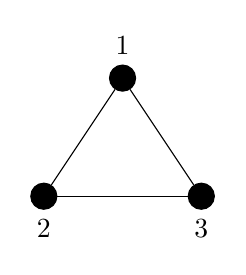
\begin{tikzpicture}
						\node [draw, circle, fill = black, label = above:1] (a) at (1, 1.5) {};
						\node [draw, circle, fill = black, label = below:2] (b) at (0, 0  ) {};
						\node [draw, circle, fill = black, label = below:3] (c) at (2, 0  ) {};
						\draw (a) to (b);
						\draw (a) to (c);
						\draw (b) to (c);
					\end{tikzpicture}
				\end{center}
				it just disappears, dropping the connections to the second and third qubit:
				\begin{center}
					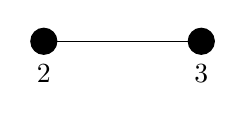
\begin{tikzpicture}
						\node [draw, circle, fill = black, label = below:2] (b) at (0, 0  ) {};
						\node [draw, circle, fill = black, label = below:3] (c) at (2, 0  ) {};
						\draw (b) to (c);
					\end{tikzpicture}
				\end{center}
				Similar rules exist for other measurements, but these are again out of scope for this course.
			% end
		% end

		\subsection{Multi-Qubit Gates}
			\label{subsec:multiQubitGates}

			So far, we only discussed local gates acting on a single qubit (remember, gates combined with tensor products are applied on each gate individually). While this already allows some calculations, it does not allow interplay of multiple qubits or generation of entangled states which are very important for various protocols (see \autoref{sec:protocols}). Hence, we need \emph{multi-qubit gates} \(U\) that cannot be written as the product of local gates, i.e., \( U \neq U_1 \otimes \dots \otimes U_N \).

			\paragraph{CNOT-Gate}
				The simplest is the CNOT-gate:
				\begin{align}
					\begin{aligned}
						\Qcircuit @C=1em @R=1em {
							\lstick{\ket{x}} & \ctrl{1} & \rstick{\ket{x}}          \qw \\
							\lstick{\ket{y}} & \targ    & \rstick{\ket{x \oplus y}} \qw
						}
					\end{aligned}
					&&
					\CNOT_{12} =
						\begin{bmatrix}
							1 & 0 & 0 & 0 \\
							0 & 1 & 0 & 0 \\
							0 & 0 & 0 & 1 \\
							0 & 0 & 1 & 0
						\end{bmatrix}
					&&
					\begin{tabular}{c|c}
						\textbf{Input} & \textbf{Output} \\ \midrule
						 \(\ket{00}\)  &  \(\ket{00}\)   \\
						 \(\ket{01}\)  &  \(\ket{01}\)   \\
						 \(\ket{10}\)  &  \(\ket{11}\)   \\
						 \(\ket{11}\)  &  \(\ket{10}\)
					\end{tabular}
				\end{align}
				This gate is a \emph{controlled} gate and applied the X-gate to the second qubit iff the first qubit is \(1\). The indices \(\CNOT_{ij}\) indicate that the gate is acting on the \(j\)-th qubit (the \emph{target}) and controlled by the \(i\)-th qubit. This gate can be extended to more than two qubits (with \(n - 1\) control qubits and a single target). For \(n = 3\), it is called the \emph{Toffoli gate} which can be used to represent classical logical operations like logical not, and, or, and not-and.
			% end

			\paragraph{SWAP-Gate}
				Another important two-qubit gate is the SWAP-gate
				\begin{align}
					\begin{aligned}
						\Qcircuit @C=1em @R=1.5em {
							\lstick{\ket{a}} & \qswap      & \rstick{\ket{b}} \qw \\
							\lstick{\ket{b}} & \qswap \qwx & \rstick{\ket{a}} \qw
						}
					\end{aligned}
					&&
					\begin{aligned}
						\Qcircuit @C=1em @R=1em {
							\lstick{\ket{a}} & \ctrl{1} & \targ     & \ctrl{1} & \rstick{\ket{b}} \qw \\
							\lstick{\ket{b}} & \targ    & \ctrl{-1} & \targ    & \rstick{\ket{b}} \qw \\
						}
					\end{aligned}
				\end{align}
				which simply switches the state of two qubits. The circuit on the right is the implementation of the SWAP-gate. Showing their equivalence is straightforward:
				\begin{align}
					\ket{00}
						\overset{\CNOT_{12}}{\longto} \ket{00}
						\overset{\CNOT_{21}}{\longto} \ket{00}
						\overset{\CNOT_{12}}{\longto} \ket{00}
					&&
					\ket{01}
						\overset{\CNOT_{12}}{\longto} \ket{01}
						\overset{\CNOT_{21}}{\longto} \ket{11}
						\overset{\CNOT_{12}}{\longto} \ket{10}
					\\
					\ket{10}
						\overset{\CNOT_{12}}{\longto} \ket{11}
						\overset{\CNOT_{21}}{\longto} \ket{01}
						\overset{\CNOT_{12}}{\longto} \ket{01}
					&&
					\ket{11}
						\overset{\CNOT_{12}}{\longto} \ket{10}
						\overset{\CNOT_{21}}{\longto} \ket{10}
						\overset{\CNOT_{12}}{\longto} \ket{11}
				\end{align}
				As unitary transformations are linear, we almost always only have to show the equivalence for the basis states as every state can be expressed as a superposition of them. This simplifies a lot of derivations! As the above circuit implements swapping for the basis states, it is a valid implementation of the SWAP-gate.
			% end

			\paragraph{Controlled-U-Gate}
				Note that any gate \(U\) can be used in a controlled fashion:
				\begin{align}
					\begin{aligned}
						\Qcircuit @C=1em @R=1em {
							\lstick{\ket{x}} & \ctrl{1} & \rstick{\ket{x}}     \qw \\
							\lstick{\ket{y}} & \gate{U} & \rstick{U^x \ket{y}} \qw
						}
					\end{aligned}
					&&
					\mathit{CU}_{12} =
						\begin{bmatrix}
							\ID & 0 \\
							0   & U
						\end{bmatrix}
				\end{align}
				To implement this gate in practice, it can be decomposed into CNOT-gates and single-qubit gates (see \autoref{subsubsec:controlledUnitaries}).
			% end

			\paragraph{Preparing the Bell State}
				Equipped with these tools, we can prepare the Bell state \(\ket{\Phi^+}\) with the following circuit:
				\begin{align}
					\begin{aligned}
						\Qcircuit @C=1em @R=1em {
							\lstick{\ket{0}}_1 & \gate{H} & \ctrl{1} & \qw \\
							\lstick{\ket{0}}_2 & \qw      & \targ    & \qw
						}
					\end{aligned}
					&&
					\ket{00}
						\overset{H_1}{\longto} \frac{1}{\sqrt{2}} (\ket{0} + \ket{1}) \ket{0}
						\overset{\CNOT_{12}}{\longto} \frac{1}{\sqrt{2}} (\ket{00} + \ket{11}) = \ket{\Phi^+}
				\end{align}
				For brevity, we will write
				\begin{equation}
					\Qcircuit @C=1em @R=1em {
						\lstick{\ket{0}} & \multigate{1}{\Phi^+} & \qw \\
						\lstick{\ket{0}} & \ghost{\Psi^+}        & \qw
					}
				\end{equation}
				from now on whenever a Bell state is prepared between two qubits. Also, we will leave out the explicit derivation of the Bell state will from derivations.
			% end
		% end
	% end

	\section{Protocols}
		\label{sec:protocols}

		In this section we discuss some essential protocols in \ac{QC} and the no-cloning theorem. These protocols are not complete algorithms (which are discussed in \autoref{c:algorithms}), but illustrate essential ideas supporting some of the algorithms.

		\subsection{No-Cloning}
			While the no-cloning theorem is not really a protocol, it is an extremely important result for \ac{QC} and thus also covered here.

			\begin{theorem}[No-Cloning]
				Let \(\ket{\psi}\) be some state. Then there exists no \(U\) such that \( U \ket{\psi} \ket{0} = \ket{\psi}\ket{\psi} \). That is, no circuit exists that copies an arbitrary quantum state.
			\end{theorem}
			\begin{proof}
				Assume that \(U\) is a cloning circuit and let \(\ket{\psi}\) and \(\ket{\phi}\) be arbitrary states. Then we can compute
				\begin{equation}
					(\bra{\phi}\bra{\phi}) (\ket{\psi}\ket{\psi})
						= \ip{\phi}{\psi} \ip{\psi}{\phi}
						= (\ip{\phi}{\psi})^2.
				\end{equation}
				However, we can also express the composite states as \( \ket{\phi}\ket{\phi} = U \ket{\phi}\ket{0} \) and \( \ket{\psi}\ket{\psi} = U \ket{\psi}\ket{0} \) using the definition of the cloning circuit \(U\). Hence,
				\begin{equation}
					\bra{0}\bra{\phi} \underbrace{U^\dagger U}_{= \ID} \ket{\psi}\ket{0}
						= \bra{0}\bra{\phi} \ket{\psi}\ket{0}
						= \ip{0}{0} \ip{\phi}{\psi}
						= \ip{\phi}{\psi}.
				\end{equation}
				Therefore, \( (\ip{\phi}{\psi})^2 = \ip{\phi}{\psi} \) holds. The states \(\ket{\phi}\) and \(\ket{\psi}\) are therefore orthogonal, \( \ip{\phi}{\psi} = 0 \), or equal, \( \ip{\phi}{\psi} = 1 \). This corresponds to classical data (either \num{0} or \num{1}) and no arbitrary quantum states. Hence, there exists no such \(U\).
			\end{proof}

			This theorem is a fundamental result of \ac{QC} and hinders some algorithms down the line. But it is not new! In fact, the no-cloning theorem is \emph{equivalent} to Heisenberg's uncertainty principles stating that for any quantum system there exist two properties which cannot both be measured with certainty. Proofing this equivalence would go as follows (proofing both directions using contraposition):
			\begin{itemize}
				\item From no-cloning to Heisenberg: if Heisenberg's uncertainty principle would be false, we could measure everything with certainty and thus prepare a second state simply by transferring the measured data, violating the no-cloning theorem.
				\item From Heisenberg to no-cloning: if the no-cloning theorem would be false, we could copy an arbitrary quantum state an arbitrary number of times and thus measure the state with arbitrary precision, violating Heisenberg's uncertainty principle.
			\end{itemize}
		% end

		\subsection{Quantum Teleportation}
			With \emph{quantum teleportation,} it is possible to teleport an arbitrary quantum state from one position to another (e.g., from Alice's to Bob's lab) using entanglement. Both parties (Alice and Bob) previously shared a Bell state \(\ket{\Phi^+}\) and now Alice wants to transmit her state \(\ket{\psi}\) over to Bob, but they cannot meet and have no secure communication channel. However, Alice can publicly announce two classical bits of information that Bob will read.

			Consider the following circuit:
			\begin{equation}
				\Qcircuit @C=1em @R=1em {
					\lstick{\ket{\psi}} & \ustick{A'} \qw & \qw                   & \ctrl{1} & \gate{H} & \meter & \ustick{m_2} \cw         & \cw \cwx[2]    &                         \\
					\lstick{\ket{0}}    & \ustick{A}  \qw & \multigate{1}{\Phi^+} & \targ    & \qw      & \meter & \ustick{m_1} \cw \cwx[1] &                &                         \\
					\lstick{\ket{0}}    & \ustick{B}  \qw & \ghost{\Phi^+}        & \qw      & \qw      & \qw    & \gate{X^{m_1}}           & \gate{Z^{m_2}} & \rstick{\ket{\psi}} \qw
				}  \label{eq:teleportation}
			\end{equation}
			Note how the state \(\ket{\psi}\) is teleported from qubit \(A\) to qubit \(B\). Also note that the state is not cloned as Alice's measurement destroys her copy. To see that the above circuit actually copies the state, we can simply calculate what it does to the circuit. Let \( \ket{\psi} = c_0 \ket{0} + c_1 \ket{1} \) be the qubit to be copied. Right before the measurements, the system has the following state:
			\begin{align}
					&\quad (c_0 \ket{0} + c_1 \ket{1})_{A'} \ket{00}_{AB} \\
				\prescript{\Phi^+_{AB}}{}{\longto}
					&\quad \frac{1}{\sqrt{2}} (c_0 \ket{0} + c_1 \ket{1})_{A'} (\ket{00} + \ket{11})_{AB} \\
				\prescript{\CNOT_{A' A}}{}{\longto}
					&\quad \frac{1}{\sqrt{2}} \bigl( c_0 \ket{0}_{A'} (\ket{00} + \ket{11})_{AB} + c_1 \ket{1}_{A'} (\ket{10} + \ket{01})_{AB} \bigr) \\
				\prescript{H_{A'}}{}{\longto}
					&\quad \frac{1}{\sqrt{2}} \bigl( c_0 \ket{+}_{A'} (\ket{00} + \ket{11})_{AB} + c_1 \ket{-}_{A'} (\ket{10} + \ket{01})_{AB} \bigr) \\
				   =&\quad \frac{1}{2} \bigl( c_0 (\ket{0} + \ket{1})_{A'} (\ket{00} + \ket{11})_{AB} + c_1 (\ket{0} - \ket{1})_{A'} (\ket{10} + \ket{01})_{AB} \bigr) \\
				   =&\quad \frac{1}{2} \bigl(
							  \ket{00}_{A' A} (c_0 \ket{0} + c_1 \ket{1})_B
							+ \ket{01}_{A' A} (c_0 \ket{1} + c_1 \ket{0})_B \\&\quad\qquad\qquad
							+ \ket{10}_{A' A} (c_0 \ket{0} - c_1 \ket{1})
							+ \ket{11}_{A' A} (c_0 \ket{1} - c_1 \ket{0})_B
						\bigr)
			\end{align}
			When now measuring the first two qubits, the following outcomes and post-measurement states are present, and the corresponding corrections have to be applied to recover \(\ket{\psi}\):
			\begin{center}
				\centering
				\begin{tabular}{cc|c|c}
					\(m_1\) & \(m_2\) &        \(\ket{\psi'}_B\)        & Correction \\ \midrule
					 \(0\)  &  \(0\)  & \( c_0 \ket{0} + c_1 \ket{1} \) &  \(\ID\)   \\
					 \(0\)  &  \(1\)  & \( c_0 \ket{1} + c_1 \ket{0} \) &   \(X\)    \\
					 \(1\)  &  \(0\)  & \( c_0 \ket{0} - c_1 \ket{1} \) &   \(Z\)    \\
					 \(1\)  &  \(1\)  & \( c_0 \ket{1} - c_1 \ket{0} \) &   \(ZX\)
				\end{tabular}
			\end{center}
			With \( U^1 = U \) and \( U^0 = \ID \), the corrections can be summarized into \( Z^{m_2} X^{m_1} \) which are the last two gates of circuit \eqref{eq:teleportation}.

			We therefore teleported a qubit from A to B! Note that this does \emph{not} allow transmission of information faster-than-light as the two classical bits have to be transmitted. Without them, the qubit is worthless as Bob cannot interpret it correctly\footnote{One might argue that Bob might get lucky and read out the correct information. But this kind of "faster-than-light transportation" is also possible classically: you can just guess what the information is---but does not actually transmit information!}. It also does not violate the no-cloning theorem as Alice's copy is destroyed during the measurement.

			\subsubsection{Concatenated Teleportation}
				\todo{Concatenated Teleportation; ???}
			% end
		% end

		\subsection{Dense-Coding}
			We are now concerned with the "opposite" problem of qubit teleportation: instead of teleporting a qubit's state, we physically transport it to another location but encode two classical bits of information in it. That is, we transmit two bits of classical information by only transmitting a single qubit. Consider the following circuit:
			\begin{equation}
				\Qcircuit @C=1em @R=1em {
					\lstick{\ket{0}} & \ustick{A} \qw & \multigate{1}{\Phi^+} & \gate{U} & \ctrl{1} & \gate{H} & \meter & \rstick{m_1} \cw \\
					\lstick{\ket{0}} & \ustick{B} \qw & \ghost{\Phi^+}        & \qw      & \targ    & \qw      & \meter & \rstick{m_2} \cw
				}
			\end{equation}
			After creating the Bell state, Alice applies a unitary \( U \in \{ \ID, X, Z, ZX \} \) and subsequently transmits the qubit to Bob. He, now in possession of both qubits \(A\) and \(B\), now applies the rest of the gates to read out what unitary Alice applied. The measurement results are as follows:
			\begin{center}
				\begin{tabular}{c|cc}
					 \(U\)  & \(m_1\) & \(m_2\) \\ \midrule
					\(\ID\) &  \(0\)  &  \(0\)  \\
					 \(X\)  &  \(0\)  &  \(1\)  \\
					 \(Z\)  &  \(1\)  &  \(0\)  \\
					\(ZX\)  &  \(1\)  &  \(1\)
				\end{tabular}
			\end{center}
			Validating this is analogous to the teleportation and left as an exercise to the reader.

			Again, this protocol does not allow faster-than-light communication as the qubit has to be physically transmitted. A combination with the teleportation protocol is possible, but this in turns requires the classical transmission of two bits, so still no faster-than-light transmission is possible.
		% end
	% end

	\section{Why these postulates?}
		One might ask \emph{why} the postulates are as is (e.g., Why probabilities in the first place? Why amplitudes and not real positive numbers? Why the Euclidean norm and not an arbitrary \(p\)-norm? Why linearity?). The hard way to understand this is:
		\begin{enumerate}
			\item learn classical physics
			\item learn why classical physics is not sufficient
			\item learn quantum physics
			\item maybe hear about why amplitudes and not probabilities
		\end{enumerate}
		However, this course is not the place to squeeze in at least one year worth of lectures just to understand the postulates. Instead, we will take a more pragmatic approach, starting from why we use the Euclidean norm.

		\paragraph{Why the Euclidean Norm?}
			Consider \( \vec{v} = (v_1, v_2, \dots, v_N) \) describing the probabilities of an event with \(N\) possible outcomes. We impose a condition \( \lVert \vec{v} \rvert_p = 1 \) to ensure normalization. The most natural choice would be \( p = 1 \), i.e., requiring that the sum of the magnitudes is unity. However, remember that we want to apply transformations \(\mat{A}\) to the vector and still keep the normalization condition: \( \lVert \vec{v} \rVert_p = \lVert \mat{A} \vec{v} \rVert_p = 1 \). For any \(p\), this condition only allows permutations \( v_i \mapsto v_j \) and sign flips \( v_i \mapsto -v_i \). None of these are capable of encoding everything interesting! However, for \( p \in \{ 1, 2 \} \), these matrices can encode more things. For \( p = 1 \), stochastic matrices are allows and for \( p = 2 \), we can use unitary matrices! For higher \(p\), no interesting behavior can be encoded. A very practical argument why we use \(p = 2\) is therefore that otherwise \ac{QM} would be very boring.
		% end

		\paragraph{Why Complex Numbers?}
			Again, we can bring up a very practical argument: only complex number are algebraically closed. Consider, for instance, a unitary gate \(U\). Applying this gate takes \(t\) time. If we want to apply it for only \(t/2\) time, we need to take its square-root \( U = VV = V^2 \). With being closed under this operation, it might be that there is no such gate! But as we are able to apply it for only \(t/2\) time, there must be some form of square-root-\(U\) in the universe. Hence, we have to use complex numbers. Take, for instance, the gate \( U = Z = \diag(1, -1) = \bigl(\diag(1, i)\bigr)^2 \).
		% end

		\paragraph{Why Linearity?}
			We always have the assumption that gates progress our state linearly. If it would not, i.e., if it would progress nonlinearly, we could solve NP-complete problems! But this is unrealistic, so we confine ourselves to linear evolution\dots
		% end

		\paragraph{What is Quantum Mechanics About?}
			Quantum mechanics is not about matter, energy, waves, nor particles. Instead, its solely about information, probabilities, and observables and how these relate to each other! Whenever seeing two linear operators in \ac{QM}, the sole answer to whether they commute conveys large amounts of information.
		% end
	% end
% end

\chapter{Computational Complexity}
	In this chapter we cover the basic ideas of complexity theory. As the core motivation behind \ac{QC} is to speed up certain tasks, we first have to lay the ground for discussing what "speed up" actually means. In computer science, the \emph{complex} of an algorithm describes the resources required to run it. This resource is often \emph{space} or \emph{time.} That is, how much memory or time it takes to run a specific algorithm. To assign a complexity to a problem instead of a specific algorithm, we assign say that the problem has the complexity of the best algorithm solving it.

	The most common complexity classes are depicted in \autoref{fig:complexityZoo}. These are:
	\begin{itemize}
		\item P: problems that are solvable in polynomial time (graph connectivity, testing if a number is prime, matchmaking, sorting, linear search, \dots)
		\item \ac{BQP}: problems solvable on a quantum computer with bounded error probability (e.g., \( P(\text{error}) \leq 2/3 \)) (factoring, discrete logarithm, \dots?)
		\item NP: problems believed to not be solvable in polynomial time (graph isomorphism, \dots)
		\item NP-complete: hard problems that can be reduced on each other and for which the solution can be checked in polynomial time (box packing, map coloring, traveling salesman, \(n \times n\) Sudoku, \dots)
		\item PSPACE: problems which need polynomial amount of memory (\(n \times n\) chess, \(n \times n\) Go, \dots)
	\end{itemize}
	These complexity classes are defined such that \(\text{P} \subseteq \text{BQP} \subseteq \text{NP} \subseteq \text{PSPACE}\). A big open problem of computer science is whether \( \text{P} \neq \text{NP} \), i.e., whether we can solve all problems "fast." A similar question comes up for \ac{QC}: is \( \text{P} \neq \text{BQP} \), i.e., are there problems that can actually be solved faster on a quantum computer?

	To assess the complexity of a quantum algorithm, we count the gates required to implement the circuit. We will see in the next chapter (\autoref{c:universality}) how this scales with the problem size.

	\begin{figure}
		\centering
		\begin{tikzpicture}[class/.style = { minimum height = 0.75cm }]
			\def\dist{0.25cm};

			\node [class, draw, circle, inner sep = \dist] (p) {P};
			\node [class, right = 1 of p] (bqp) {BQP};
			\node [class, right = 1 of bqp] (np) {NP};
			\node [class, right = 1 of np, draw, circle, inner sep = \dist] (npComplete) {NP-Complete};
			\node [class, right = 1 of npComplete] (pspace) {PSPACE};

			\path (p.west) to coordinate(b) (bqp.east);
			\path (p.west) to coordinate(c) (np.east);
			\draw let \p1 = ($(p.west) - (b)$), \n1 = {veclen(\x1, \y1)} in (b) node[draw, circle, minimum width = 2*(\n1+1*\dist)](b){};
			\draw let \p1 = ($(p.west) - (c)$), \n1 = {veclen(\x1, \y1)} in (c) node[draw, circle, minimum width = 2*(\n1+2*\dist)](c){};
			\path let \p1 = (c.west),      \p2 = (c.north) in coordinate[xshift = -\dist, yshift =  \dist](A) at (\x1, \y2);
			\path let \p1 = (pspace.east), \p2 = (c.north) in coordinate[xshift = +\dist, yshift =  \dist](B) at (\x1, \y2);
			\path let \p1 = (pspace.east), \p2 = (c.south) in coordinate[xshift = +\dist, yshift = -\dist](C) at (\x1, \y2);
			\path let \p1 = (c.west),      \p2 = (c.south) in coordinate[xshift = -\dist, yshift = -\dist](D) at (\x1, \y2);
			\draw (A) to (B) to (C) to (D) to cycle;
		\end{tikzpicture}
		\caption{The Computational Complexity Zoo}
		\label{fig:complexityZoo}
	\end{figure}
% end

\chapter{Universal Computation}
	\label{c:universality}

	In general, a quantum circuit is just a unitary \(U\) and measurements,
	\begin{equation}
		\Qcircuit @C=1em @R=1em {
			\lstick{\ket{x_1}} & \multigate{3}{U} & \meter \\
			\lstick{\ket{x_2}} & \ghost{U}        & \meter \\
			\lstick{\raisebox{5.5pt}{\vdots}}    & \ghost{U}        & \rstick{\raisebox{4.8pt}{\vdots}} \qw \\
			\lstick{\ket{x_n}} & \ghost{U}        & \meter
		}
	\end{equation}
	with an initialization \( \ket{x_1 x_2 \dots x_n} \). However, this circuit has to be constructed somehow from gates we have available in the lab. this raises the natural question of what gates we have to implement to build every unitary---and whether there are actually a set of gates fulfilling this.

	\begin{definition}[Universal Set of Gates]
		A set of gates \(\mathcal{G}\) is called \emph{universal} if any unitary can be approximated with arbitrary accuracy using only gates from this set. With a gate \(U\) and its approximation \(V\), let
		\begin{equation}
			E(U, V) = \max_{\ket{\psi}}\; \lVert (U - V) \ket{\psi} \rVert
		\end{equation}
		be the \emph{error} between \(U\) and \(V\). Note that this error is an upper bound on the probability error \( \lvert P_U - P_V \rvert \leq 2 E(U, V) \) quantifying the difference in the probability distributions induced by applying \(U\) or \(V\) to a state.
	\end{definition}

	Note that is analogous to classical computing. There we could also decompose every algorithm into a set of universal logical gates. For instance, the sets \( \{\, \text{AND}, \text{OR}, \text{NOT} \,\} \) and \( \{\, \text{NAND} \,\} \) are both universal and can represent every possible classical circuit. We formulate this into a theorem:

	\begin{theorem}[Classical Set of Universal Gates]  \label{th:classicalUniversal}
		The sets \( \{\, \text{AND}, \text{OR}, \text{NOT} \,\} \) and \( \{\, \text{NAND} \,\} \) and universal for all classical logic gates.
	\end{theorem}
	\begin{proof}
		By induction.
	\end{proof}

	\begin{theorem}[Embedding of Classical Circuits]
		Every classical circuit can be embedded in a quantum circuit performing the equivalent operation, but reversibly.
	\end{theorem}
	\begin{proof}
		To proof this, we use that \( \{\, \text{AND}, \text{NOT}, \text{OR} \,\} \) is universal for all classical gates (\autoref{th:classicalUniversal}). We therefore only have to show that these gates can be resembled using quantum circuits. For this, we use the X-, CNOT-, and Toffoli-gate:
		\begin{align}
			\begin{aligned}
				\Qcircuit{
					\lstick{\ket{x}} & \ctrl{2} & \rstick{\ket{x}} \qw \\
					\lstick{\ket{y}} & \ctrl{1} & \rstick{\ket{y}} \qw \\
					\lstick{\ket{0}} & \targ    & \rstick{\ket{x \land y}} \qw
				}
			\end{aligned}
			&&
			\begin{aligned}
				\Qcircuit{
					\lstick{\ket{x}} & \ctrl{1} & \rstick{\ket{y}} \qw \\
					\lstick{\ket{1}} & \targ    & \rstick{\ket{\lnot x}} \qw
				}
			\end{aligned}
			&&
			\begin{aligned}
				\Qcircuit @C=1em @R=1em {
					\lstick{\ket{x}} & \gate{X} & \ctrl{1} & \gate{X} & \rstick{\ket{x}} \qw \\
					\lstick{\ket{y}} & \gate{X} & \ctrl{1} & \gate{X} & \rstick{\ket{y}} \qw \\
					\lstick{\ket{1}} & \qw      & \targ    & \qw      & \rstick{\ket{x \lor y}} \qw
				}
			\end{aligned}
		\end{align}
		Showing the equivalence is trivial. Note that in the logical or, the Toffoli-gate functions as a not-and due to the target qubit being set to \(\ket{1}\).
	\end{proof}

	\section{Universal Quantum Gates}
		In this section we will go over the proof of universality. Some common groups of quantum gates that are discussed are, for instance, the \emph{Pauli group} \( \mathcal{P} = \langle X, Z \rangle \) from which all the Pauli-gates can be constructed:
		\begin{equation}
			\langle X, Z \rangle
				\longto \{ X^2 = Z^2 = \ID, X, XZ = iY, ZX = -iY, Z \}
				\equiv \{ \ID, X, Y, Z \}.
		\end{equation}
		Another important group is the \emph{Clifford group} \( \mathcal{C} = \langle H, S, \CNOT \rangle \) with
		\begin{equation}
			\langle H, S, \CNOT \rangle
				\longto \{ H^2 = \ID, S^2 = Z, \dots \}.
		\end{equation}
		However, we have the following result:
		\begin{theorem}[Gottesman-Knill Theorem]
			Circuits build using solely gates from the Clifford group can be efficiently simulated on a classical computer.
		\end{theorem}
		Hence, the Clifford group is not enough as we will never see a speedup when just using its gates! However, if we add the T-gate \( T = \diag(1, e^{i \pi / 4}) \), we get a universal set of gates:
		\begin{theorem}[Universal Set of Quantum Gates]
			The following set of quantum gates is universal: \( \langle H, S, \CNOT, T \rangle \).
		\end{theorem}
		\begin{proof}[Proof Sketch]
			The proof of this theorem has three parts:
			\begin{enumerate}
				\item every unitary matrix can be decomposed into the product of two-level\footnote{A two-level unitary matrix is a matrix that only acts non-trivially on at most two vector components.} unitary matrices
				\item every two-level unitary matrix can be decomposed into CNOT- and single-qubit gates
				\item every single-qubit gate can be approximated with arbitrary accuracy by \( \langle H, T \rangle \)
			\end{enumerate}
			which we will cover in greater detail.

			\emph{Part 1/3:}  \todo{Universality Proof: Part 1/3; 4.16}
			For an \(n\)-qubit gate \(U\), at most \( 2^{n - 1} (2^n - 1) \in \mathcal{O}(4^n) \) two-level unitary matrices are needed.

			\emph{Part 2/3:}
			Let \(\tilde{U} \in \C^{2{n + 1} \times 2^{n + 1}}\) be a two-level unitary matrix acting on \(n + 1\) qubits. Assume w.l.o.g. that \(\tilde{U}\) is a block diagonal matrix \( \tilde{U} = \diag(\ID, U) \), where \( U \in \C^{2 \times 2} \) contains the four non-trivial entries of \(\tilde{U}\). Hence, \(\tilde{U}\) is a the \(n\)-controlled version of \(U\), i.e., \(U\) is only applied to the \((n + 1)\)-th qubit iff the first \(n\) qubits are \num{1}. To show that this gate can be constructed using just single-qubit gates and CNOT-gates, we first construct a controlled-U-gate, then a controlled-controlled-U-gate, and subsequently expand this to an \(n\)-controlled-U-gate.

			Let \( U \eqqcolon e^{i \alpha} A X B X C \) be a decomposition of \(U\) such that \( A B C = \ID \) (note that this is always possible due to \autoref{th:twoByTwoDecomposition}). The following circuit implements a controlled-U-gate:
			\begin{equation}
				\Qcircuit @C=1em @R=1em {
					& \qw      & \ctrl{1} & \qw      & \ctrl{1} & \gate{E} & \qw \\
					& \gate{C} & \targ    & \gate{B} & \targ    & \gate{A} & \qw
				}
			\end{equation}
			with \( E \coloneqq \diag(1, e^{i \alpha}) \). For \(\ket{0x}\), both \(E\) and the CNOT-gates have no effect and therefore due to \(A B C = \ID\), the state is left as is. For \(\ket{1x}\), both \(E\) and the CNOT-gates are applied and therefore the unitary \(C X B X A\) acts on the second qubit together with the global phase \(e^{i \alpha}\), which is equivalent to applying \(U\). Similarly,
			\begin{equation}
				\Qcircuit @C=1em @R=1em {
					& \qw              & \ctrl{1} & \qw              & \ctrl{1} & \gate{E^\dagger} & \qw \\
					& \gate{A^\dagger} & \targ    & \gate{B^\dagger} & \targ    & \gate{C^\dagger} & \qw
				}
			\end{equation}
			implements the controlled-\(U^\dagger\)-gate necessary for the next step (the proof is analogous).

			The controlled-controlled-U-gate is realized by
			\begin{equation}
				\Qcircuit @C=1em @R=1em {
					& \qw      & \ctrl{1} & \qw              & \ctrl{1} & \ctrl{2} & \qw \\
					& \ctrl{1} & \targ    & \ctrl{1}         & \targ    & \qw      & \qw \\
					& \gate{V} & \qw      & \gate{V^\dagger} & \qw      & \gate{V} & \qw
				}  \label{eq:ccu}
			\end{equation}
			with \(V\) being the half-U-gate, i.e., \( V^2 = U \). For \(\ket{00x}\), no gate is ever applied. For \(\ket{01x}\), \(V\) and \(V^\dagger\) are applied, canceling each other out. For \(\ket{10x}\), \(V^\dagger\) and \(V\) are applied, canceling each other out. For \(\ket{11x}\), however, both \(V\) but not \(V^\dagger\) are applied (due to the CNOT-gates canceling the activation on the second qubit), resulting in \(VV = V^2 = U\) being applied to the this qubit. Hence, this circuit realizes the controlled-controlled-U-gate. By some clever arrangement, this circuit needs eight single-qubit gates and six CNOT-gates.

			To build the \(n\)-controlled-U-gate, we add the new control bits to the front and expand the control lines of \eqref{eq:ccu} to these qubits, using an \((n - 1)\)-controlled-gate. Finally, we end up using \( \mathcal{O}(n^2) \) CNOT- and single-qubit gates.
			\todo{Universality Proof: Part 2/3: Why don't we need exponentially many gates here, too?}

			\emph{Part 3/3:}  \todo{Universality Proof: Part 3/3; 4.21}
%			By the triangle inequality, error of multiple gates accumulate linearly, i.e.,
%			\begin{equation}
%				E(U_n \dots U_2 U_1, V_n \dots U_2 U_1) \leq \sum_{i = 1}^{n} E(U_i, V_i).
%			\end{equation}
%			With the decomposition \( U = R_{\hat{n}}(\delta) R_{\hat{m}}(\gamma) R_{\hat{n}}(\beta) \)
			By the \emph{Solovay-Kitaev theorem,} approximating a circuit with \(m\) CNOT- and single-qubit up to an accuracy \(\epsilon\) requires \( \mathcal{O}\bigl( m \log^2(m / \epsilon) \bigr) \) gates from \( \langle H, T \rangle \).

			This concludes the proof sketch and we end up with
			\begin{equation}
				\mathcal{O}\Biggl( 4^n 2^n \log^2\biggl( \frac{4^n 2^n}{\epsilon} \biggr) \Biggr)
			\end{equation}
			gates to approximate an arbitrary \(n\)-qubit quantum circuit.
		\end{proof}

		From this discussion and the final gate count that scales exponentially with the number of qubit, it does not appear clear why anyone should think that \( \text{BQP} \neq \text{P} \). Even classical circuits need an exponential amount of time on a quantum computer! This is the reason why algorithms that are efficient on a quantum computer are rare and require a large amount of creativity. The next chapter covers nearly all quantum algorithms that we know so far, which only reinforces the argument how much creativity is necessary to invent new ones.
	% end
% end

\chapter{Algorithms} % 5.3
	\label{c:algorithms}

	\todo{Content}

	\section{Quantum Parallelism} % 5.4, 5.5
		\todo{Content}

		\subsection{Interference} % 5.6, 5.7
			\todo{Content}
		% end

		\subsection{The Query Unitary} % 6.4, 6.5, 6.6, 6.21
			\todo{Content}
		% end

		\subsection{Deutsch's Approach} % 5.8, 5.9, 5.10
			\todo{Content}
		% end
	% end

	\section{Deutsch-Josza Algorithm} % 5.11, 5.12, 5.13, 5.14, E6.2, E6.3
		\todo{Content}
	% end

	\section{Bernstein-Vazirani Algorithm} % 5.15, 5.16, 5.17, 5.22, 5.23, 5.24, 5.25, 5.18, 6.8
		\todo{Content}
	% end

	\section{Simon's Algorithm} % 6.11, 6.21, E6.4
		\todo{Content}

		\subsection{Problem} % 6.12, 6.13
			\todo{Content}
		% end

		\subsection{Classical Approach} % 6.13, 6.14
			\todo{Content}
		% end

		\subsection{Quantum Approach} % N/A
			\todo{Content}

			\subsubsection{Circuit} % 6.15, 6.16, 6.17, 6.18
				\todo{Content}
			% end

			\subsubsection{Post-Processing} % 6.18, 6.19
				\todo{Content}
			% end

			\subsubsection{Remarks} % 6.20
				\todo{Content}
			% end
		% end
	% end

	\section{Quantum Fourier Transform} % 8.6, 8.7
		\todo{Content}

		\subsection{Binary Fraction Expansion} % 8.7, 8.8, 8.20, 8.21
			\todo{Content}
		% end

		\subsection{Quantum Circuit} % 8.8, 8.9, 8.10, E7.1, E7.3, E8.2
			\todo{Content}
		% end

		\subsection{Remarks} % 8.11
			\todo{Content}
		% end
	% end

	\section{Shor's Algorithm} % 7.3, 7.4, 7.5, 7.6
		\todo{Content}

		\subsection{Period Finding} % 7.7, 7.8, 7.9, 7.10, 7.23, 8.3, 8.4
			\todo{Content}

			\subsubsection{Using Quantum Fourier Transform} % 7.11, 7.12, 7.13, 7.14, 7.15
				\todo{Content}
			% end

			\subsubsection{Post-Processing} % 7.16
				\todo{Content}

				\paragraph{Maximizing the \(P(y)\)} % 7.17, 7.18
					\todo{Content}
				% end

				\paragraph{Recovering the Period} % 7.19, 7.20, 7.21
					\todo{Content}
				% end

				\paragraph{Remarks} % 7.22
					\todo{Content}
				% end
			% end
		% end

		\subsection{From Period Finding to Factoring} % 8.12, 8.13, 8.14, 8.15, 8.16
			\todo{Content}

			\subsubsection{Remarks} % 8.17
				\todo{Content}
			% end
		% end

		\subsection{Summary} % 8.18, 8.19
			\todo{Content}
		% end
	% end

	\section{Grover's Algorithm} % 9.2, 9.3, 9.25, E9.1, E9.2
		\todo{Content}

		\subsection{Classical Approach} % 9.7
			\todo{Content}
		% end

		\subsection{Quantum Approach} % 9.7, 9.8
			\todo{Content}

			\subsubsection{Circuit} % 9.9, 9.10, 9.11
				\todo{Content}

				\paragraph{Illustration} % 9.12, 9.15, 9.16, 9.17, 9.18, 9.19, 9.20
					\todo{Content}
				% end

				\paragraph{Algebraic Proof} % 9.13, 9.14
					\todo{Content}
				% end
			% end

			\subsubsection{Multiple Solutions} % 9.21, 9.22
				\todo{Content}
			% end

			\subsubsection{Remarks} % 9.23, 9.24
				\todo{Content}
			% end
		% end
	% end
% end

\chapter{Quantum Error Correction}
	So far, we assumed that applying gates works perfectly, i.e., that the state transform exactly as our mathematical model predicts. However, in the real world, (quantum) computers are noisy and by no means perfect. In classical computing, the errors that might occur when sending a message (e.g., through the internet or through time by saving it to disk) are confined to bit-flips. In order to make a computer resilient towards bit-flips, the most simplistic approach is to just copy the data and define \emph{logical bits}
	\begin{align}
		0 &\mapsto 000 \eqqcolon 0_L &
		1 &\mapsto 111 \eqqcolon 1_L.
	\end{align}
	This is called \emph{encoding} and the protocol is called the \emph{code} (in this case, \emph{repetition} code). Decoding the message works by a majority vote, i.e.:
	\begin{align}
		000 &\mapsto 0 &
		001 &\mapsto 0 &
		010 &\mapsto 0 &
		011 &\mapsto 1 \\
		100 &\mapsto 0 &
		101 &\mapsto 1 &
		110 &\mapsto 1 &
		111 &\mapsto 1
	\end{align}
	This means that a decoding error happens only if more than one bit is flipped. In other words: the encoding is resilient w.r.t. to one bit-flip. Assume that a bit-flip happens with probability \(p\) (see \autoref{fig:bitFlipChannelClassical}). Then the error probability is
	\begin{equation}
		p_e^{(1)} \coloneqq P(\text{two or more flipped})
			= 3 P(\text{exactly two flipped}) + P(\text{all flipped})
			= 3 p^2 (1 - p) + p^3
			< 3p^2,
	\end{equation}
	where \( 3p^2 \) is an upper bound. If we re-apply the encoding (and therefore encode a logical bit into nine physical bits), the new error probability is \( p_e^{(2)} = 3 (3p^2)^2 \). In general, after \(k\) applications of the encoding, the error probability is proportional to \( (3p)^{2^k} \). Hence, \( (3p)^{2^k} \to_{k \to \infty} 0 \) for \(p < 1/3\) and we can achieve an arbitrarily good encoding for finite \(k\).

	But can we directly transfer this principle to \ac{QEC}? No, because:
	\begin{itemize}
		\item We cannot copy data due to the no-cloning theorem---but would it even help as measurements destroy everything anyway?
		\item We do not have discrete error but a continuum---do we need infinite precision to locate the error?
		\item Measuring destroys the message---how to do decode?
	\end{itemize}
	Fortunately though, all of these problems can be circumvented and \ac{QEC} is possible. We will now cover two kinds of errors: bit-flips and phase-flips and will subsequently see that correcting these suffices to correct all possible errors, effectively reducing the continuum of errors to a finite set.

	\begin{figure}
		\centering
		\begin{subfigure}[b]{0.3\linewidth}
			\centering
			\begin{tikzpicture}[->]
				\node (a) {\(0\)};
				\node [below = 1 of a] (b) {\(1\)};
				\node [right = 3 of a] (c) {\(0\)};
				\path let \p1 = (c), \p2 = (b) in node (d) at (\x1, \y2) {\(1\)};
				\draw (a) to node[above]{\( 1 - p \)} (c);
				\draw (a) to node[above, pos = 0.4]{\( p \)} (d);
				\draw (b) to node[below, pos = 0.4]{\( p \)} (c);
				\draw (b) to node[below]{\( 1 - p \)} (d);
			\end{tikzpicture}
			\caption{Classical Bit-Flip}
			\label{fig:bitFlipChannelClassical}
		\end{subfigure}
		~
		\begin{subfigure}[b]{0.3\linewidth}
			\centering
			\begin{tikzpicture}[->]
				\node (a) {\(\ket{\psi}\)};
				\node [below = 1 of a] (b) {};
				\node [right = 3 of a] (c) {\(\ket{\psi}\)};
				\path let \p1 = (c), \p2 = (b) in node (d) at (\x1, \y2) {\(X \ket{\psi}\)};
				\draw (a) to node[above]{\( 1 - p \)} (c);
				\draw (a) to node[above, pos = 0.4]{\( p \)} (d);
			\end{tikzpicture}
			\caption{Quantum Phase-Flip}
			\label{fig:bitFlipChannelQuantum}
		\end{subfigure}
		~
		\begin{subfigure}[b]{0.3\linewidth}
			\centering
			\begin{tikzpicture}[->]
				\node (a) {\(\ket{\psi}\)};
				\node [below = 1 of a] (b) {};
				\node [right = 3 of a] (c) {\(\ket{\psi}\)};
				\path let \p1 = (c), \p2 = (b) in node (d) at (\x1, \y2) {\(Z \ket{\psi}\)};
				\draw (a) to node[above]{\( 1 - p \)} (c);
				\draw (a) to node[above, pos = 0.4]{\( p \)} (d);
			\end{tikzpicture}
			\caption{Quantum Bit-Flip}
			\label{fig:phaseFlipChannelQuantum}
		\end{subfigure}
		\caption[Bit/Phase-Flip Channels]{State diagram for classical/quantum bit/phase-flip channels while sending a message. A bit/phase-flip happens with probability \(p\) and the message is left untouched with probability \(1 - p\).}
		\label{fig:flipChannel}
	\end{figure}

	\section{Tackling Bit-Flips}
		We start by fixing bit-flips. To encode the message, we copy the coefficients of an arbitrary state \( \ket{\psi} = \alpha \ket{0} + \beta \ket{1} \) to two encoding qubits:
		\begin{equation}
			\begin{aligned}
				\Qcircuit @C=1em @R=1em {
					\lstick{\ket{\psi}} & \ctrl{1} & \ctrl{2} & \qw \\
					\lstick{\ket{0}}    & \targ    & \qw      & \qw \\
					\lstick{\ket{0}}    & \qw      & \targ    & \qw
				}
			\end{aligned}
			= \alpha \ket{000} + \beta \ket{000}
			\eqqcolon \alpha \ket{0}_L + \beta \ket{1}_L
		\end{equation}
		Note that we did not actually copy the state, but only the \emph{coefficients} which does not violate the no-cloning theorem! We now assume that an error only happens on exactly one qubit (because otherwise we are not able to recover anyway). We encode this as follows:
		\begin{align}
			\begin{aligned}
				\Qcircuit @C=1em @R=1em {
					\lstick{\ket{\psi}} & \ctrl{1} & \ctrl{2} & \gate{X^i} & \qw \\
					\lstick{\ket{0}}    & \targ    & \qw      & \gate{X^j} & \qw \\
					\lstick{\ket{0}}    & \qw      & \targ    & \gate{X^k} & \qw
				}
			\end{aligned}
			&&
			\begin{tabular}{ccc|c}
				\(i\) & \(j\) & \(k\) & State                                    \\ \midrule
				\(0\) & \(0\) & \(0\) & \( \alpha \ket{000} + \beta \ket{111} \) \\
				\(1\) & \(0\) & \(0\) & \( \alpha \ket{100} + \beta \ket{011} \) \\
				\(0\) & \(1\) & \(0\) & \( \alpha \ket{010} + \beta \ket{101} \) \\
				\(0\) & \(0\) & \(1\) & \( \alpha \ket{001} + \beta \ket{110} \)
			\end{tabular}
		\end{align}
		Fortunately, all possible result states are orthogonal! Hence, we can uniquely identify my measuring even though they are all in superposition. However, if we would simply measure, we would destroy the state. We therefore copy the state again into two \emph{helper qubits} which we can then measure:
		\begin{align}
			\begin{aligned}
				\Qcircuit @C=1em @R=1em {
					\lstick{\ket{\psi}} & \ctrl{1} & \ctrl{2} & \gate{X^i} & \ctrl{3} & \qw      & \qw      & \qw      & \qw    & \multigate{2}{C}     & \qw \\
					\lstick{\ket{0}}    & \targ    & \qw      & \gate{X^j} & \qw      & \ctrl{2} & \ctrl{3} & \qw      & \qw    & \ghost{C}            & \qw \\
					\lstick{\ket{0}}    & \qw      & \targ    & \gate{X^k} & \qw      & \qw      & \qw      & \ctrl{2} & \qw    & \ghost{C}            & \qw \\
					                    &          &    & \lstick{\ket{0}} & \targ    & \targ    & \qw      & \qw      & \meter & \rstick{x} \cw \cwx  & \\
					                    &          &    & \lstick{\ket{0}} & \qw      & \qw      & \targ    & \targ    & \meter & \rstick{y} \cw \cwx  &
				}
			\end{aligned}
			&&
			\begin{tabular}{cc|c}
				\(x\) & \(y\) & Correction \(C\) \\ \midrule
				\(0\) & \(0\) &     \(\ID\)      \\
				\(0\) & \(1\) &     \(X_3\)      \\
				\(1\) & \(0\) &     \(X_1\)      \\
				\(1\) & \(1\) &     \(X_2\)
			\end{tabular}
		\end{align}
		The interpretation of this is as follows: for \(x = 1\), we conclude that the first and second qubit have different values. Similarly, \(y = 1\) encodes that the second and third qubit have different values. If they have the same value, the CNOT-gates would either be not applied or cancel each other out. Note again that the sole reason why this works is that the state are orthogonal! From this discussion, we can deduce the above corrections.

		This approach is also called a \emph{parity check} of \(Z_1 Z_2\) and \(Z_2 Z_3\), i.e., a parity check in Z-basis.
	% end

	\section{Tackling Phase-Flips}
		Correcting phase-flips (see \autoref{fig:phaseFlipChannelQuantum}) is analogous to correcting bit-flips, but in Hadamard basis. The encoding circuit including the error model along with the resulting states therefore is:
		\begin{align}
			\begin{aligned}
				\Qcircuit @C=1em @R=1em {
					\lstick{\ket{\psi}} & \ctrl{1} & \ctrl{2} & \gate{H} & \gate{Z^i} & \qw \\
					\lstick{\ket{0}}    & \targ    & \qw      & \gate{H} & \gate{Z^j} & \qw \\
					\lstick{\ket{0}}    & \qw      & \targ    & \gate{H} & \gate{Z^k} & \qw
				}
			\end{aligned}
			&&
			\begin{tabular}{ccc|c}
				\(i\) & \(j\) & \(k\) & State                                    \\ \midrule
				\(0\) & \(0\) & \(0\) & \( \alpha \ket{+++} + \beta \ket{---} \) \\
				\(1\) & \(0\) & \(0\) & \( \alpha \ket{-++} + \beta \ket{+--} \) \\
				\(0\) & \(1\) & \(0\) & \( \alpha \ket{+-+} + \beta \ket{-+-} \) \\
				\(0\) & \(0\) & \(1\) & \( \alpha \ket{++-} + \beta \ket{--+} \)
			\end{tabular}
		\end{align}
		By applying Hadamard again in the decoding circuit, the identity \( H Z H = X \) directly tells us that we need to apply the same corrections as for bit-flips:
		\begin{align}
			\begin{aligned}
				\Qcircuit @C=1em @R=1em {
					\lstick{\ket{\psi}} & \ctrl{1} & \ctrl{2} & \gate{H} & \gate{Z^i} & \gate{H} & \ctrl{3} & \qw      & \qw      & \qw      & \qw    & \multigate{2}{C}     & \qw \\
					\lstick{\ket{0}}    & \targ    & \qw      & \gate{H} & \gate{Z^j} & \gate{H} & \qw      & \ctrl{2} & \ctrl{3} & \qw      & \qw    & \ghost{C}            & \qw \\
					\lstick{\ket{0}}    & \qw      & \targ    & \gate{H} & \gate{Z^k} & \gate{H} & \qw      & \qw      & \qw      & \ctrl{2} & \qw    & \ghost{C}            & \qw \\
					                    &          &          &          &    & \lstick{\ket{0}} & \targ    & \targ    & \qw      & \qw      & \meter & \rstick{x} \cw \cwx  & \\
					                    &          &          &          &    & \lstick{\ket{0}} & \qw      & \qw      & \targ    & \targ    & \meter & \rstick{y} \cw \cwx  &
				}
			\end{aligned}
			&&
			\begin{tabular}{cc|c}
				\(x\) & \(y\) & Correction \(C\) \\ \midrule
				\(0\) & \(0\) &     \(\ID\)      \\
				\(0\) & \(1\) &     \(X_3\)      \\
				\(1\) & \(0\) &     \(X_1\)      \\
				\(1\) & \(1\) &     \(X_2\)
			\end{tabular}
		\end{align}
		This approach is a parity check of \(X_1 X_2\) and \(X_2 X_3\), i.e., a parity check in X-basis.

		\todo{QEC: The lecture says that phase-flips should be corrected by applying Z-gates---but why???}
	% end

	\section{Shor's Code}
		The idea of \emph{Shor's code} is to concatenate the circuits discussed before, using the bit-flip correction three times for each physical qubit of the phase-flip parity check. The whole circuit is shown in \autoref{fig:shorsCode}. One can easily verify that Shor's code used the following mapping for logical qubits:
		\begin{equation}
			\begin{aligned}
				\ket{0} &\mapsto \frac{\ket{000} + \ket{111}}{\sqrt{2}} \otimes \frac{\ket{000} + \ket{111}}{\sqrt{2}} \otimes \frac{\ket{000} + \ket{111}}{\sqrt{2}} \eqqcolon \ket{0}_L \\
				\ket{1} &\mapsto \frac{\ket{000} - \ket{111}}{\sqrt{2}} \otimes \frac{\ket{000} - \ket{111}}{\sqrt{2}} \otimes \frac{\ket{000} - \ket{111}}{\sqrt{2}} \eqqcolon \ket{1}_L
			\end{aligned}
			\label{eq:shorCode}
		\end{equation}
		An important feature of Shor's code is that it is not only capable of correcting \(X\) or \(Z\) errors, but also \(XZ\) errors, i.e., simultaneous bit- and phase-flips. With this feature, it is possible to correct any possible error (see \autoref{subsec:universalQEC}). However, Shor's code is not optimal as it uses so many qubits. It is also possible to use only seven or even five qubits, see \autoref{subsec:otherCodes}.

\begin{figure}
	\centering
\begin{equation}
\resizebox{0.9\linewidth}{!}{
\Qcircuit @C=1em @R=1em {
\lstick{\ket{\psi}_1} & \ctrl{5} & \ctrl{10} & \gate{H} &        \qw         & \ctrl{1} & \ctrl{2} &    \gate{X^i}    & \gate{Z^\ell}    & \ctrl{3} &   \qw    &   \qw    &   \qw    &  \qw   & \multigate{2}{C_1}    & \gate{H} & \ctrl{15} &    \qw    &    \qw    &    \qw    &   \qw    &   \qw    &    \qw    &    \qw    &   \qw    &   \qw    &   \qw    &   \qw    & \qw &  \qw   &   \multigate{12}{C}  & \qw \\
&          &           &          & \lstick{\ket{0}_2} &  \targ   &   \qw    &    \gate{X^j}    & \gate{Z^m}       &   \qw    & \ctrl{2} & \ctrl{3} &   \qw    &  \qw   & \ghost{C_1}           & \gate{H} &    \qw    & \ctrl{14} &    \qw    &    \qw    &   \qw    &   \qw    &    \qw    &    \qw    &   \qw    &   \qw    &   \qw    &   \qw    & \qw &  \qw   &       \ghost{C}      & \qw \\
&          &           &          & \lstick{\ket{0}_3} &   \qw    &  \targ   &    \gate{X^k}    & \gate{Z^n}       &   \qw    &   \qw    &   \qw    & \ctrl{2} &  \qw   & \ghost{C_1}           & \gate{H} &    \qw    &    \qw    & \ctrl{13} &    \qw    &   \qw    &   \qw    &    \qw    &    \qw    &   \qw    &   \qw    &   \qw    &   \qw    & \qw &  \qw   &       \ghost{C}      & \qw \\
&          &           &          &                    &          &          &                  & \lstick{\ket{0}} &  \targ   &  \targ   &   \qw    &  \qw     & \meter & \rstick{x_1} \cw \cwx &          &           &           &           &           &          &          &           &           &          &          &          &          &     &        &                      &     \\
&          &           &          &                    &          &          &                  & \lstick{\ket{0}} &   \qw    &   \qw    &  \targ   &  \targ   & \meter & \rstick{y_1} \cw \cwx &          &           &           &           &           &          &          &           &           &          &          &          &          &     &        &                      &     \\
\lstick{\ket{0}_4}   &  \targ   &    \qw    & \gate{H} &        \qw         & \ctrl{1} & \ctrl{2} &    \gate{X^i}    & \gate{Z^\ell}    & \ctrl{3} &   \qw    &   \qw    &   \qw    &  \qw   & \multigate{2}{C_2}    & \gate{H} &    \qw    &    \qw    &    \qw    & \ctrl{10} &   \qw    &   \qw    & \ctrl{11} &    \qw    &   \qw    &   \qw    &   \qw    &   \qw    & \qw &  \qw   &       \ghost{C}      & \qw \\
&          &           &          & \lstick{\ket{0}_5} &  \targ   &   \qw    &    \gate{X^j}    & \gate{Z^m}       &   \qw    & \ctrl{2} & \ctrl{3} &   \qw    &  \qw   & \ghost{C_2}           & \gate{H} &    \qw    &    \qw    &    \qw    &    \qw    & \ctrl{9} &   \qw    &    \qw    & \ctrl{10} &   \qw    &   \qw    &   \qw    &   \qw    & \qw &  \qw   &       \ghost{C}      & \qw \\
&          &           &          & \lstick{\ket{0}_6} &   \qw    &  \targ   &    \gate{X^k}    & \gate{Z^n}       &   \qw    &   \qw    &   \qw    & \ctrl{2} &  \qw   & \ghost{C_2}           & \gate{H} &    \qw    &    \qw    &    \qw    &    \qw    &   \qw    & \ctrl{8} &    \qw    &    \qw    & \ctrl{9} &   \qw    &   \qw    &   \qw    & \qw &  \qw   &       \ghost{C}      & \qw \\
&          &           &          &                    &          &          &                  & \lstick{\ket{0}} &  \targ   &  \targ   &   \qw    &   \qw    & \meter & \rstick{x_2} \cw \cwx &          &           &           &           &           &          &          &           &           &          &          &          &          &     &        &                      &     \\
&          &           &          &                    &          &          &                  & \lstick{\ket{0}} &   \qw    &   \qw    &  \targ   &  \targ   & \meter & \rstick{y_2} \cw \cwx &          &           &           &           &           &          &          &           &           &          &          &          &          &     &        &                      &     \\
\lstick{\ket{0}_7}   &   \qw    &   \targ   & \gate{H} &        \qw         & \ctrl{1} & \ctrl{2} &    \gate{X^i}    & \gate{Z^\ell}    & \ctrl{3} &   \qw    &   \qw    &   \qw    &  \qw   & \multigate{2}{C_3}    & \gate{H} &    \qw    &    \qw    &    \qw    &    \qw    &   \qw    &   \qw    &    \qw    &    \qw    &   \qw    & \ctrl{6} &   \qw    &   \qw    & \qw &  \qw   &       \ghost{C}      & \qw \\
&          &           &          & \lstick{\ket{0}_8} &  \targ   &   \qw    &    \gate{X^j}    & \gate{Z^m}       &   \qw    & \ctrl{2} & \ctrl{3} &   \qw    &  \qw   & \ghost{C_3}           & \gate{H} &    \qw    &    \qw    &    \qw    &    \qw    &   \qw    &   \qw    &    \qw    &    \qw    &   \qw    &   \qw    & \ctrl{5} &   \qw    & \qw &  \qw   &       \ghost{C}      & \qw \\
&          &           &          & \lstick{\ket{0}_9} &   \qw    &  \targ   &    \gate{X^k}    & \gate{Z^n}       &   \qw    &   \qw    &   \qw    & \ctrl{2} &  \qw   & \ghost{C_3}           & \gate{H} &    \qw    &    \qw    &    \qw    &    \qw    &   \qw    &   \qw    &    \qw    &    \qw    &   \qw    &   \qw    &   \qw    & \ctrl{4} & \qw &  \qw   &       \ghost{C}      & \qw \\
&          &           &          &                    &          &          &                  & \lstick{\ket{0}} &  \targ   &  \targ   &   \qw    &   \qw    & \meter & \rstick{x_3} \cw \cwx &          &           &           &           &           &          &          &           &           &          &          &          &          &     &        &         \cwx         &     \\
&          &           &          &                    &          &          &                  & \lstick{\ket{0}} &   \qw    &   \qw    &  \targ   &  \targ   & \meter & \rstick{y_3} \cw \cwx &          &           &           &           &           &          &          &           &           &          &          &          &          &     &        &         \cwx         &     \\
&          &           &          &                    &          &          &                  & \lstick{\ket{0}} &   \qw    &   \qw    &   \qw    &   \qw    &  \qw   & \qw                   &   \qw    &   \targ   &   \targ   &   \targ   &   \targ   &  \targ   &  \targ   &    \qw    &    \qw    &   \qw    &   \qw    &   \qw    &   \qw    & \qw & \meter &  \rstick{x} \cw \cwx &     \\
&          &           &          &                    &          &          &                  & \lstick{\ket{0}} &   \qw    &   \qw    &   \qw    &   \qw    &  \qw   & \qw                   &   \qw    &    \qw    &    \qw    &    \qw    &    \qw    &   \qw    &   \qw    &   \targ   &   \targ   &  \targ   &  \targ   &  \targ   &  \targ   & \qw & \meter &  \rstick{y} \cw \cwx &
}
}
		\end{equation}
		\caption[Shor's Code]{Quantum circuit for encoding in Shor's code (the left part until the error gates \(X\) and \(Z\)) and for decoding (everything to the right of the error gates). The matrices \(C_1\), \(C_2\), \(C_3\), and \(C\) denote the corresponding correction matrices for the bit flip ("inner" code) and the phase flip ("outer" code).}
		\label{fig:shorsCode}
\end{figure}

		\subsection{Universal Error Correction}
			\label{subsec:universalQEC}

			As already discussed is the Shor code capable of correcting \(XZ\)-type errors acting on a single qubit. From this we can conclude that the Shor code is in fact capable of correcting arbitrary errors, even non-unitary ones, as long as they act on a single qubit and are valid quantum operations.

			\begin{theorem}[Universal Error Correct]
				The Shor code is capable of correcting arbitrary errors.
			\end{theorem}
			\begin{proof}
				W.l.o.g, assume that the error happens on the first qubit and is described by \( E_1 \in \C^{2 \times 2} \). We can express this matrix using the three Pauli matrices:
				\begin{equation}
					E = \alpha_0 \ID_1 + \alpha_1 X_1 + \alpha_2 Z_1 + \alpha_3 X_1 Z_1
				\end{equation}
				This is easy to verify by calculating the right-hand-side, equating it to \(E_1\), and explicitly solving the resulting linear system of equations:
				\begin{equation}
					\begin{bmatrix}
						e_{11} & e_{21} \\
						e_{21} & e_{22}
					\end{bmatrix}
					=
					\begin{bmatrix}
						\alpha_0 + \alpha_2 & \alpha_1 - \alpha_3 \\
						\alpha_1 + \alpha_3 & \alpha_0 - \alpha_2
					\end{bmatrix}
					\qquad\implies\qquad
					\begin{bmatrix}
						\alpha_0 \\
						\alpha_1 \\
						\alpha_2 \\
						\alpha_3
					\end{bmatrix}
					=
					\frac{1}{2}
					\begin{bmatrix}
						e_{11} + e_{22} \\
						e_{12} + e_{21} \\
						e_{11} - e_{22} \\
						e_{21} - e_{12}
					\end{bmatrix}
				\end{equation}
				Let \( \ket{\psi}_L = \alpha \ket{0}_L + \beta \ket{1}_L \) be a logical qubit encoded with Shor's code (see \eqref{eq:shorCode} for the logical basis states). Then, by linearity, an application of the error operator \(E_1\) yields
				\begin{equation}
					E_1 \ket{\psi}_L = \alpha_0 \ket{\psi}_L + \alpha_1 X_1 \ket{\psi}_L + \alpha_2 Z_1 \ket{\psi}_L + \alpha_3 X_1 Z_1 \ket{\psi}_L.
				\end{equation}
				By dropping the last six qubits from the basis states (as the error only acts on the first qubit), each individual error has the following effect on \( \ket{\psi}_K \):
				\begin{align}
					  \ID_1 \ket{\psi}_L &= \frac{\alpha}{\sqrt{2}} (\ket{000} + \ket{111}) \otimes \ket{\cdots} + \frac{\beta}{\sqrt{2}} (\ket{000} - \ket{111}) \otimes \ket{\cdots} \\
					    X_1 \ket{\psi}_L &= \frac{\alpha}{\sqrt{2}} (\ket{100} + \ket{011}) \otimes \ket{\cdots} + \frac{\beta}{\sqrt{2}} (\ket{100} - \ket{011}) \otimes \ket{\cdots} \\
					    Z_1 \ket{\psi}_L &= \frac{\alpha}{\sqrt{2}} (\ket{000} - \ket{111}) \otimes \ket{\cdots} + \frac{\beta}{\sqrt{2}} (\ket{000} + \ket{111}) \otimes \ket{\cdots} \\
					X_1 Z_1 \ket{\psi}_L &= \frac{\alpha}{\sqrt{2}} (\ket{100} - \ket{011}) \otimes \ket{\cdots} + \frac{\beta}{\sqrt{2}} (\ket{100} + \ket{011}) \otimes \ket{\cdots}
				\end{align}
				As these states are mutually orthogonal, measuring the parity qubits uniquely identifies one of the four errors and the state collapses onto either one of them. Subsequently, Shor's code can be used to correct the individual errors. Hence, Shor's code can be used to correct arbitrary errors.
			\end{proof}
		% end
	% end

	\section{Other Codes}
		\label{subsec:otherCodes}

		As already mentioned, the Shor code is not \emph{optimal} in the sense of saving qubits. There exist several smaller ones, for instance the \emph{Steane code}
		\begin{align}
			\ket{0}_L &= \frac{1}{\sqrt{8}} (\ket{0000000} + \ket{1010101} + \ket{0110011} + \ket{1100110} + \ket{0001111} + \ket{1011010} + \ket{0111100} + \ket{1101001}) \\
			\ket{1}_L &= \frac{1}{\sqrt{8}} (\ket{1111111} + \ket{0101010} + \ket{1001100} + \ket{0011001} + \ket{1110000} + \ket{0100101} + \ket{1000011} + \ket{0010110})
		\end{align}
		or five-qubit codes. However, the Steane code has some nice properties which we will discuss in the next section.
	% end

	\section{Fault-Tolerance and Transversality} % 10.18, 10.19, 10.20, 10.21, 10.22, 10.23, E10.3
		\label{subsec:faultTolerance}

		In fault-tolerant \ac{QC}, the idea is to perform all operations in encoded states (i.e., logical qubits), without ever decoding. One code supporting this is the Steane code we saw in the previous section. It allows us to execute certain gates \emph{transversely.} That is, we can design a gate that has the same effect on the individual physical qubits as on the logical qubits. For the Steane code, the basic gates are simply tensor-products of single-qubit gates:
		\begin{align}
			X_L &= X_1 \otimes X_2 \otimes \dots \otimes X_7 &
			Z_L &= Z_1 \otimes Z_2 \otimes \dots \otimes Z_7 &
			H_L &= H_1 \otimes H_2 \otimes \dots \otimes H_7
		\end{align}
		While they acting on the individual qubits is trivial, one can also show that:
		\begin{align}
			X_L \ket{0}_L &=  \ket{1}_L &
			X_L \ket{1}_L &=  \ket{0}_L \\
			Z_L \ket{0}_L &=  \ket{0}_L &
			Z_L \ket{1}_L &= -\ket{1}_L \\
			H_L \ket{0}_L &= \frac{1}{\sqrt{2}} (\ket{0}_L + \ket{1}_L) = \ket{+}_L &
			H_L \ket{1}_L &= \frac{1}{\sqrt{2}} (\ket{0}_L - \ket{1}_K) = \ket{-}_L
		\end{align}
		An important property to consider in fault-tolerant \ac{QC} is how errors propagate. For the X-gate, for instance, an error does not propagate to other physical qubits as the gate is local and can be corrected with the Steane code. Application of a CNOT-gate withing a Steane block, however, may propagate an error onto a second qubit which can not be corrected! Instead, a logical CNOT-gate
		\begin{equation}
			\CNOT_L \ket{x}_L \ket{y}_L \mapsto \ket{x}_L \ket{x \oplus y}_L = \CNOT_{1, 8} \otimes \CNOT_{2, 9} \otimes \dots \otimes \CNOT_{7, 14}
		\end{equation}
		has to be used that only works across two blocks (see \autoref{fig:logicalCnot} for the circuit). The T-gate, however, cannot be implemented transversely. Its fault-tolerant implementation is more complicated and out of scope for this course.
		\todo{Fault-Tolerance: Proof that T-gate cannot be implemented transversely.}

		The general scheme of performing fault-tolerant \ac{QC} is:
		\begin{enumerate}
			\item prepare quantum state in logical qubit
			\item apply fault-tolerant gate
			\item correct errors
			\item go to second step until the algorithm is finished
		\end{enumerate}
		As we already saw, the second step is the fundamental challenge as it is hard to come up with fault-tolerant gates, which we define as follows:
		\begin{definition}[Fault-Tolerance]
			A procedure is called \emph{fault-tolerant} if the failure of one component causes at most one error in each encoded block at the output step.
		\end{definition}

		\begin{figure}
			\centering
			\begin{equation}
				\Qcircuit @C=2em @R=0.25em @!R {
					& \ctrl{8} & \qw & \qw & \qw & \qw & \qw & \qw & \qw \\
					& \qw & \ctrl{8} & \qw & \qw & \qw & \qw & \qw & \qw \\
					& \qw & \qw & \ctrl{8} & \qw & \qw & \qw & \qw & \qw \\
					& \qw & \qw & \qw & \ctrl{8} & \qw & \qw & \qw & \qw \\
					& \qw & \qw & \qw & \qw & \ctrl{8} & \qw & \qw & \qw \\
					& \qw & \qw & \qw & \qw & \qw & \ctrl{8} & \qw & \qw \\
					& \qw & \qw & \qw & \qw & \qw & \qw & \ctrl{8} & \qw \\
					&&&&&&&& \\
					& \targ & \qw & \qw & \qw & \qw & \qw & \qw & \qw \\
					& \qw & \targ & \qw & \qw & \qw & \qw & \qw & \qw \\
					& \qw & \qw & \targ & \qw & \qw & \qw & \qw & \qw \\
					& \qw & \qw & \qw & \targ & \qw & \qw & \qw & \qw \\
					& \qw & \qw & \qw & \qw & \targ & \qw & \qw & \qw \\
					& \qw & \qw & \qw & \qw & \qw & \targ & \qw & \qw \\
					& \qw & \qw & \qw & \qw & \qw & \qw & \targ & \qw \\
				}
			\end{equation}
			\caption{Fault-Tolerant CNOT-Gate}
			\label{fig:logicalCnot}
		\end{figure}
	% end

	\section{Threshold Theorem}
		So far, we assumed that the \ac{QEC} itself works perfectly. But what if the error correction itself causes errors again? Like for classical repetition codes, we can simply re-encode the bits, building up a layered coding architecture. Let \(m\) be the number of places where an error can occur, then the probability of an error using a single coding layer is upper-bounded by \( p_e^{(1)} = (mp)^2 \). For \(k\) layers, the error probability is \( p_e^{(k)} = (mp)^{2^k} \) which, analogous to classical error correction, converges to zero for \(k \to \infty\) if \(p < 1/m\). Hence, we can achieve any error probability \(\epsilon\) with a large enough \(k\).

		This brings us to the \emph{threshold theorem:}
		\begin{theorem}[Threshold Theorem]
			A quantum circuit with \(p(n)\) gates on \(n\) qubits may be simulated with an error probability of at most \(\epsilon > 0\) using\footnote{Note that in the lecture, this bound is written as \( \mathcal{O}\bigl( p(n) \, \mathrm{poly}( \log(p(n)/\epsilon) ) \bigr) \).}
			\begin{equation}
				\mathcal{O}\Biggl( p(n) \, \log^c \frac{p(n)}{\epsilon} \Biggr)
			\end{equation}
			gates (for some constant \(c\) when the gates fail with probability of at most \(p\) given that \(p < p_\mathrm{th}\) for some code-dependent constant threshold \(p_\mathrm{th}\).
		\end{theorem}
		For the Steane code, \( p_\mathrm{th} \approx 10^{-5} \). Hence, to factor numbers with around \num{2000}, we would needs millions of millions of qubits! This is the sole reason why we do not have quantum computing at the moment!
		% TODO: Look again at the theshold theorem.
	% end
% end

\chapter{Quantum Nonlocality} % 11.3
	\label{c:nonlocality}

	\todo{Content}

	\section{Elements of Reality} % 11.4, 11.5, 11.6, 11.7, 11.8, 11.9, 11.10
		\todo{Content}
	% end

	\section{CHSH Inequality} % 11.12, 11.13, 11.14, 11.15
		\todo{Content}
	% end

	\section{Quantum Violation of the CHSH Inequality} % 11.16, 11.17, 11.21
		\todo{Content}
	% end

	\section{Tsirelson's Bound and Quantum Key Distribution} % 11.22, 11.23, 11.24, 11.25
		\todo{Content}
	% end
% end

\chapter{Measurement-Based Quantum Computing} % 12.1, 12.9, 12.10, 12.11, 12.12, 12.25
	\todo{Content}

	\section{Identity} % 12.13, 12.14
		\todo{Content}
	% end

	\section{Arbitrary Rotations} % 12.15, 12.16, 12.17
		\todo{Content}
	% end

	\section{CNOT} % 12.18
		\todo{Content}
	% end

	\section{Cluster States} % 12.19, 12.20
		\todo{Content}
	% end

	\section{Handling Errors} % 12.20, 12.21, 12.22, 12.23, 12.24
		\todo{Content}
	% end

	\section{Important Gates} % ???, E3.2, E3.3
		\todo{Content}
	% end
% end
